%% Elsevier CAS double-column template.
%% cas-dc loads xcolor WITHOUT the table option; pass it here so that
%% \rowcolors (alternating row shading) is available in every table.
\PassOptionsToPackage{table}{xcolor}
%% allow long URLs to break across lines in the first-page footnote
\PassOptionsToPackage{hyphens}{url}
\documentclass[a4paper,fleqn]{cas-dc}

\usepackage[numbers]{natbib}
\usepackage{booktabs}
\usepackage{graphicx}
\usepackage{multirow}
\usepackage{makecell}
\usepackage{rotating}
\usepackage{pifont}
\newcommand{\cmark}{\ding{51}}
\newcommand{\xmark}{\ding{55}}
\newcommand{\pmark}{$\circ$}
\newcommand{\rotbox}[1]{\rotatebox{90}{\scriptsize #1}}

%% ---- table conventions -------------------------------------------------
%% Alternating row shading: \zebra{n} starts the banding at body row n of
%% the tabular (rows are counted from the first row after \begin{tabular},
%% header rows included), so each table declares where its body begins.
%% ROW n IS ALWAYS THE FIRST SHADED ROW, whatever its parity. This needs the
%% \ifodd below, and without it the banding phase is silently wrong: xcolor's
%% \rowcolors{n}{odd}{even} keys off each row's ABSOLUTE number, not off an
%% offset from n, so plain \rowcolors{n}{}{rowshade} shades row n only when n
%% is even. With a one-line header (\zebra{2}) that happened to be right; with
%% a two-line header (\zebra{3}) it silently inverted, so half the tables in
%% the paper opened on a shaded body row and half on a white one, and a table
%% whose \zebra{} did not match its own header depth opened with TWO white
%% rows in a row -- which reads as a missing band rather than as a pattern.
%% ROW SHADING: ON, by the authors' decision. Noting the tension once so it is
%% a choice on the record rather than an oversight -- the Information Fusion
%% guide says "Avoid vertical rules and shading within table cells" under
%% Tables. Vertical rules we do avoid (booktabs throughout). Banding we keep,
%% because these tables are wide and read badly without a row cue. Swap the two
%% definitions below to comply literally if a referee or the production editor
%% asks.
\definecolor{rowshade}{gray}{0.94}
\newcommand{\zebra}[1]{%                             % banded (author's choice)
  \ifodd#1\relax\rowcolors{#1}{rowshade}{}\else\rowcolors{#1}{}{rowshade}\fi}
%\newcommand{\zebra}[1]{}                       % guide-literal: no cell shading
%% Better-direction markers used in column headers, the standard benchmark
%% convention: \up marks "higher is better", \down "lower is better".
%% Standard error printed beside a delta, small and grey enough that the
%% column still reads as a column of deltas rather than of pairs.
\newcommand{\sem}[1]{\,{\tiny$\pm$#1}}
\newcommand{\up}{$\uparrow$}
\newcommand{\down}{$\downarrow$}
%% ragged-right fixed-width column, so wide text columns wrap inside the
%% narrow CAS column instead of being scaled by \resizebox (which used to
%% give every table a different effective font size)
\newcolumntype{P}[1]{>{\raggedright\arraybackslash\hspace{0pt}}p{#1}}  % L/C/R are taken by makecell;
%% Stretchy first column, so every table spans its full measure instead of
%% sitting centred with a ragged band of dead space beside it. THE SLACK GOES
%% INSIDE A COLUMN, NOT INTO THE GUTTERS, and that is the whole point: the
%% obvious alternative, tabular* with @{\extracolsep{\fill}}, puts the slack in
%% inter-column glue, which \rowcolors does NOT paint -- the banding then shows
%% a white break at every column boundary (measured: a 35pt hole through the
%% shaded rows of the two-column audit table). An X column is a p-column, so
%% its background is painted like any other cell and the banding stays solid.
%% Y for a left-aligned label column, Z for a right-aligned one. Because the
%% target width exceeds the table's natural width, the X column is always
%% WIDER than its content, so nothing that fitted before can wrap now.
\usepackage{tabularx}
%% Two-line right-aligned table cell, WITHOUT a nested alignment. Table 3 needs
%% ~114 of these (a count over a per-class count) and used \makecell, which
%% typesets its content in a nested tabular. That broke the row banding in two
%% separate ways, both measured:
%%   (1) colortbl's row counter is advanced by every \cr, INCLUDING the ones
%%       inside a nested alignment. Each \makecell therefore advanced it once
%%       more, so a row carrying eleven of them advanced it twelve times and
%%       rows carrying a "x" or "--" instead advanced it fewer. The parity that
%%       \rowcolors alternates on was then effectively arbitrary: the rendered
%%       table ran six shaded rows, one white, four shaded, one white.
%%   (2) colortbl does not paint continuously behind a nested tabular, so a
%%       white seam appeared between every pair of numeric columns.
%% \mcell sets the two lines in a \parbox instead. A \parbox contains no
%% alignment, so no \cr is issued and no seam is introduced; the width is the
%% wider of the two lines, which reproduces \makecell[r]'s geometry exactly.
\newlength{\mcellw}\newlength{\mcellx}
\newcommand{\mcell}[2]{%
  \settowidth{\mcellw}{#1}%
  \settowidth{\mcellx}{#2}%
  \ifdim\mcellx>\mcellw \setlength{\mcellw}{\mcellx}\fi
  \parbox[t]{\mcellw}{\raggedleft\strut#1\par\strut#2}}
\newcolumntype{Y}{>{\raggedright\arraybackslash\hspace{0pt}}X}
\newcolumntype{Z}{>{\raggedleft\arraybackslash}X}
%% the \hspace{0pt} re-enables hyphenation of the first word, which plain
%% \raggedright suppresses (long tokens like "ImageNet-transferable" then
%% overflow no matter how the column is sized)

%% Generated numbers, derived from the run records and the audit, so a
%% number in prose cannot drift from the table beside it.
% GENERATED by scripts/make_paper_numbers.py -- do not edit.
% Every macro here is derived from the run records or the audit,
% so a number used in prose cannot drift from the table beside it.
\newcommand{\auditScope}{1{,}100}
\newcommand{\auditResolvable}{511}
\newcommand{\auditCorrect}{404}
\newcommand{\auditWrong}{107}
\newcommand{\auditUnresolved}{487}
\newcommand{\auditBracket}{102}
\newcommand{\auditRate}{79.1}
\newcommand{\auditResidSD}{2.2}  % residual spread at fixed baseline
\newcommand{\computeRuns}{8{,}827}
\newcommand{\computeGpuHours}{3{,}341}
\newcommand{\computeHhundred}{2{,}903}
\newcommand{\computeHnvl}{37}
\newcommand{\computeHtwo}{45}
\newcommand{\computeAmpere}{356}
\newcommand{\computeNvl}{82}
\newcommand{\computeKwh}{2{,}639}
\newcommand{\computeCarbon}{449}
\newcommand{\computePerRun}{51}
\newcommand{\vitBest}{75.3}  % DeiT aug + prior, CIFAR-100 100%
\newcommand{\vitBestBase}{61.4}  % same recipe without the prior
\newcommand{\vitBestDelta}{13.9}  % must equal vitBest - vitBestBase

%% tables/numbers.tex is GENERATED and must travel with the sections that quote
%% its macros. When an older copy is used -- easy to do when syncing a subset of
%% files to Overleaf -- LaTeX reports "control sequence never \def'ed" against
%% whichever macro is missing, which does not name the cause. These two checks
%% name it. Add the newest macro here whenever the generator gains one.
\makeatletter
\@ifundefined{camSigma}{\@latex@error{tables/numbers.tex is OUT OF DATE
  (\string\camSigma\space missing). Regenerate it with:
  python scripts/make_paper_numbers.py > paper/tables/numbers.tex}\@ehd}{}
\@ifundefined{numbersStamp}{\@latex@error{tables/numbers.tex is OUT OF DATE
  (no \string\numbersStamp). Regenerate it with:
  python scripts/make_paper_numbers.py > paper/tables/numbers.tex}\@ehd}{}
\@ifundefined{auditAllPaired}{\@latex@error{tables/numbers.tex is OUT OF DATE
  (\string\auditAllPaired\space missing). Regenerate it with:
  python scripts/make_paper_numbers.py > paper/tables/numbers.tex}\@ehd}{}
\makeatother

%% ---- FLOAT PLACEMENT: the real cause, found by reproducing it -----------
%% SYMPTOM (reported from Overleaf): Figures 2-10 all abandon the body and
%% pile onto float pages at the end, while every table places normally.
%%
%% HOW IT WAS FOUND. Three earlier diagnoses here were WRONG and are recorded
%% as such: it is not the [tb] specifier, not float.sty arriving with
%% \usepackage{algorithm}, and not the \@fp... float-page glue. All three were
%% inferred from a local TeX Live 2023 build that never reproduced the bug.
%% It was settled by compiling in a TeX Live 2026 container (Overleaf runs
%% 2025; local is 2023), where the fault appears immediately -- including on
%% the pristine pre-edit source, which is what proved it was never a
%% regression. In that container [tb], [tbp], [!tbp], [tp] and [htbp] all
%% produced BYTE-IDENTICAL placement. A specifier that changes nothing is not
%% being read.
%%
%% THE CAUSE. cas-common.sty does not merely style floats, it REPLACES them:
%%     \RenewDocumentEnvironment { figure } { O{} }
%%       { \__reset_fig: ... \keys_set:nn { cas / fig } { #1 }
%%         \csxdef{fps@figure}{\l_fig_pos_tl} \@float{figure} ... }
%% so the optional argument is a KEY-VALUE list (cas/fig keys: pos, width,
%% cols, align, ...), NOT a LaTeX placement specifier, and \@float is then
%% called with no optional argument at all. \__reset_fig: hard-resets the
%% position to `t' on every figure. A bare [tbp] falls to the `unknown' key
%% handler, which does \tl_set:Nn \l_fig_pos_tl {\l_keys_key_tl} -- storing
%% the macro NAME rather than its value -- so by the time \csxdef expands it
%% the intended placement is gone. Every figure in this paper had been
%% top-of-column-only, whatever the brackets said, and a top-only float with
%% nowhere to go defers until a \clearpage. `table' is defined the same way
%% and defaulted to `t' too; tables merely suffered less because they are
%% smaller.
%%
%% THE FIX: use the class's own interface, [pos=tbp], on every float. Verified
%% in the TeX Live 2026 container: figures move from a nine-figure pile-up on
%% pp. 27-31 to pp. 6-25, beside the sections that cite them, with zero float
%% warnings; the same source is equally correct on local TeX Live 2023. Write
%% [pos=...] for any float added later -- a bare [htbp] will silently do
%% nothing.
%%
%% NO placeins (its \FloatBarrier ignores \floatpagefraction and produced
%% near-empty float pages) and NO dblfloatfix (cas-dc already loads stfloats;
%% both define \c@dblbotnumber). The end-of-body \clearpage that used to guard
%% against pending floats is gone too -- with [pos=...] honoured, nothing pends.
\usepackage{flafter}                                            % never place a float before its definition
%% Pseudocode for the fusion-decision procedure. `algorithmic' ONLY -- we do
%% NOT load `algorithm'.
%% WHY, and it cost a regression to learn: algorithm.sty pulls in float.sty,
%% and float.sty does not confine itself to the float type it defines. It does
%%     \let\@float@Hx\@xfloat   \def\@xfloat#1[{...}
%% i.e. it globally reroutes \@xfloat, the core placement macro for EVERY float
%% class, in order to add its `H' specifier. cas-dc already loads stfloats,
%% which patches the double-column float lists, and we load flafter, which
%% patches \@floatplacement. Three packages plus the class all rewriting one
%% mechanism is stable only by luck, and the luck ran out on TeX Live 2025: with
%% float.sty loaded, Overleaf deferred EVERY single-column figure to float pages
%% at the end of the body (Figures 2-10 on pp. 29-33) while every table placed
%% normally -- a blocked figure queue, which is the FIFO cascade from one stuck
%% float. Local TeX Live 2023 did not reproduce it.
%% So Algorithm 1 is set inside an ordinary `table' float instead: the table
%% class is the one we can SEE placing correctly on that very Overleaf run, and
%% it needs no new float machinery. \caption is deliberately NOT used, so the
%% table counter does not advance and the float is not numbered as a Table;
%% \thealgnum supplies its own number, and \refstepcounter makes \ref work.
\usepackage{algorithmic}
\newcounter{algnum}
\renewcommand{\thealgnum}{\arabic{algnum}}
%% NO \extrafloats. It was added as insurance against "Too many unprocessed
%% floats", but it works by extending \@freelist, and \@freelist is exactly what
%% the multiply-patched float mechanism above manipulates. With [tbp] the queue
%% drains at each page break and never approached the 18-float limit in any
%% build we have measured, so the insurance was buying nothing and adding one
%% more interaction. Re-add it only if that fatal error actually appears.

%% SUBMISSION MODE. The Information Fusion guide requires the graphical
%% abstract and the highlights to be uploaded as SEPARATE files ("Submit your
%% graphical abstract as a separate file", "Submit highlights as a separate
%% editable file ... with the word highlights in the file name"), and both are
%% already listed as separate deliverables in SUBMISSION_FILES.md
%% (figs/graphical_abstract_submission.png, highlights.txt). cas-dc none the
%% less typesets each as its own prelim page, which added two pages to the
%% compiled manuscript and pushed it past the journal's 10-35 page limit for a
%% research article. Currently OFF, by the authors' decision: both pages are
%% typeset, so the compiled PDF is self-contained. Set \submissionmodetrue to
%% drop them -- they then travel as their own files (highlights.txt,
%% figs/graphical_abstract_submission.png), exactly as the guide asks, and the
%% manuscript comes back to 35 pages.
\newif\ifsubmissionmode
\submissionmodefalse
\begin{document}
\let\WriteBookmarks\relax
%% FLOAT PLACEMENT. The two lines here were previously \def\floatpagepagefraction
%% and \def\textpagefraction, neither of which is a LaTeX parameter, so the
%% intended tuning silently did nothing and floats ran on the defaults. With 32
%% floats in a two-column layout the defaults defer aggressively and push
%% figures far past the text that cites them. The single-column parameters are
%% relaxed below, and so are the DOUBLE-column ones (\dbl...), which are what
%% actually govern the full-width figure* floats.
%% These fractions were previously set as \floatpagepagefraction and
%% \textpagefraction, neither of which is a LaTeX parameter, so the tuning had
%% never taken effect. The \dbl... pair governs the full-width figure* floats,
%% which the single-column parameters do not reach.
\renewcommand{\topfraction}{0.92}
\renewcommand{\bottomfraction}{0.70}
\renewcommand{\textfraction}{0.06}
\renewcommand{\floatpagefraction}{0.70}
\renewcommand{\dbltopfraction}{0.92}
\renewcommand{\dblfloatpagefraction}{0.70}
\setcounter{topnumber}{4}
\setcounter{bottomnumber}{2}
\setcounter{totalnumber}{6}
\setcounter{dbltopnumber}{3}

%% ---- FLOAT/TEXT SEPARATION ----------------------------------------------
%% The class inherits LaTeX's defaults, and \textfloatsep is 20pt -- almost
%% exactly 2em at 10pt type -- inserted BOTH above and below every float that
%% lands at a column top or bottom. With [pos=tbp] on 37 floats that is where
%% nearly all of them land, so the document reads as though every table and
%% figure is fenced off by a blank band. \dbltextfloatsep does the same for the
%% full-width floats. Halved here, with \floatsep (float-to-float) and
%% \intextsep (in-line floats) brought down in proportion. The shrink
%% components are kept so the page breaker retains room to manoeuvre; only the
%% natural size changes.
\setlength{\textfloatsep}{10pt plus 2pt minus 3pt}
\setlength{\dbltextfloatsep}{10pt plus 2pt minus 3pt}
\setlength{\floatsep}{8pt plus 2pt minus 2pt}
\setlength{\dblfloatsep}{8pt plus 2pt minus 2pt}
\setlength{\intextsep}{8pt plus 2pt minus 2pt}

%% ---- THE SKIPS INSIDE THE FLOAT BOX -------------------------------------
%% \textfloatsep above is only half of what separates a float from the text,
%% and halving it alone left a gap that still measured 16.4pt (against a 2.7pt
%% body line gap). The other half is INSIDE the float: cas-common's
%% \__reset_fig: / \__reset_tbl: re-apply their own 6pt skips at the start of
%% EVERY float, so a preamble \setlength cannot reach them -- they have to be
%% redefined, which is what this does. Only the skips that are pure TRAILING
%% or LEADING space in the float box are zeroed:
%%   figure  = graphic, [abovecap], caption, [belowcap]   -> belowcap is trailing
%%   table   = [abovecap], caption, [abovetbl], tabular, [belowtbl]
%%                                          -> abovecap leads, belowtbl trails
%% The skips that do design work -- graphic-to-caption and caption-to-tabular
%% -- are KEPT (at 4pt, from 6pt). abovefig/belowfig are left at the class
%% default because nothing here establishes where the class applies them.
%% pos/cols/align are reproduced verbatim from cas-common so that redefining
%% these macros changes spacing and nothing else.
\ExplSyntaxOn
\cs_set:Npn \__reset_fig:
{
  \tl_set:Nx \l_fig_pos_tl { t }
  \tl_set:Nx \l_fig_cols_tl { 1 }
  \tl_set:Nn \l_fig_align_tl { \raggedleft }
  \skip_set:Nn \l_fig_abovecap_skip { 4pt }
  \skip_set:Nn \l_fig_belowcap_skip { 0pt }
  \skip_set:Nn \l_fig_abovefig_skip { 6pt }
  \skip_set:Nn \l_fig_belowfig_skip { 6pt }
}
\cs_set:Npn \__reset_tbl:
{
  \tl_set:Nx \l_tbl_pos_tl { t }
  \tl_set:Nx \l_tbl_cols_tl { 1 }
  \tl_set:Nn \l_tbl_align_tl { \centering }
  \skip_set:Nn \l_tbl_abovecap_skip { 0pt }
  \skip_set:Nn \l_tbl_belowcap_skip { 0pt }
  \skip_set:Nn \l_tbl_abovetbl_skip { 4pt }
  \skip_set:Nn \l_tbl_belowtbl_skip { 0pt }
}
\ExplSyntaxOff

%% ---- HEADING SPACING ----------------------------------------------------
%% A DELIBERATE DEVIATION FROM THE CAS TEMPLATE, and the only one in this
%% file that changes the publisher's own typography rather than fixing a
%% conflict. cas-common opens a section with 15pt and a subsection with 10pt,
%% against a 2.7pt body line gap (measured). Both are reduced by about a
%% quarter. The definitions are copied verbatim from cas-common lines
%% 1924-1935 -- same \@startsection level, indent, run-in style and font --
%% so ONLY the leading skip changes; the trailing skips (4pt and 0.1pt) are
%% untouched, since shrinking those would let a heading drift away from the
%% text it introduces. Elsevier production re-typesets to house style in any
%% case; delete this block to return to the template exactly.
\makeatletter
\renewcommand\section{\@startsection{section}{1}{\z@}%
    {11pt \@plus 3\p@ \@minus 3\p@}%
    {4\p@}%
    {\sectionfont\raggedright\hst[13pt]}}
\renewcommand\subsection{\@startsection{subsection}{2}{\z@}%
    {8pt \@plus 2\p@ \@minus 2\p@}%
    {.1\p@}%
    {\ssectionfont\raggedright}}
\renewcommand\subsubsection{\@startsection{subsubsection}{3}{\z@}%
    {8pt \@plus 1\p@ \@minus .3\p@}%
    {.1\p@}%
    {\sssectionfont\raggedright}}
\makeatother

%% ---- WHITE SPACE BEFORE AND AFTER FIGURES -------------------------------
%% Reported from Overleaf (TeX Live 2025, pdfLaTeX) and reproducible here.
%% MEASURED, not guessed. Two independent mechanisms, both fixed below.
%%
%% (1) FLOAT PAGES CENTRE THEIR CONTENT. LaTeX's defaults are
%%       \@fptop = 0pt plus 1fil   \@fpsep = 8pt plus 2fil   \@fpbot = 0pt plus 1fil
%%     -- all infinitely stretchable -- so a page made entirely of floats
%%     distributes them down the page instead of stacking them at the top. One
%%     figure on such a page is left marooned with a large white band above AND
%%     below it, which is exactly the reported symptom. This only became
%%     reachable when the floats gained `p' placement (the fix for figures
%%     spilling into the appendix), and whether a float page is built at all
%%     depends on where the page breaks fall -- which is why TeX Live 2025
%%     shows it and 2023 here did not. Removing `p' would bring the appendix
%%     spill back, so instead: kill the stretch at the TOP and keep it at the
%%     bottom, and float pages fill downward from the top margin like a normal
%%     page.
%%     \@fpsep MUST BE RIGID TOO, and the first version of this fix got that
%%     wrong. It was left at `12pt plus 1fil' with the comment "a little
%%     stretch so two floats sharing a page are not jammed together" -- but
%%     1fil is not a little stretch, it is the same infinite order as
%%     \@fpbot's, so the two split the leftover space equally. Two tables
%%     sharing a float column then sat 72.0pt apart (measured on Tables 15/16
%%     at p.19) with an equal band below, which reads as a hole between two
%%     tables. Matching \@fpsep to \floatsep makes floats on a float page
%%     stack exactly as they do on an ordinary page and sends all the slack
%%     to \@fpbot, where a short column is the normal, unremarkable outcome.
%%
%% (2) \flushbottom STRETCHES FLOAT-HEAVY COLUMNS. cas-dc sets \flushbottom
%%     (verified by probe), which forces every column to exactly \textheight by
%%     inflating the glue inside it. That is invisible on a text page, where
%%     there is plenty of inter-paragraph glue to absorb it. On a column that is
%%     mostly figure -- and \textfraction is relaxed to 0.06 here, so a column
%%     may be 94% float -- there is almost nothing to stretch except the space
%%     around the float, so the slack lands there. \raggedbottom collects the
%%     slack at the column FOOT instead, where it reads as a short column rather
%%     than as a gap wrapped around a figure. Columns may now end at slightly
%%     different heights; that is the accepted trade and is standard for
%%     figure-dense two-column papers.
\makeatletter
\setlength{\@fptop}{0pt}
\setlength{\@fpsep}{8pt plus 2pt minus 2pt}     % = \floatsep, deliberately rigid
\setlength{\@fpbot}{0pt plus 1fil}
\setlength{\@dblfptop}{0pt}
\setlength{\@dblfpsep}{8pt plus 2pt minus 2pt}  % = \dblfloatsep
\setlength{\@dblfpbot}{0pt plus 1fil}
\makeatother
%% NO \raggedbottom. It was added to stop \flushbottom inflating float-heavy
%% columns, but it also changes how much material a column accepts, which
%% feeds straight back into float placement -- and placement is the problem we
%% cannot reproduce locally. Reverted so the machinery matches the
%% configuration Overleaf placed correctly; the \@fp... glue above stays,
%% because it only governs how an already-built float PAGE is filled and
%% cannot influence whether a float is placed in a column.

\shorttitle{When does fusing knowledge with learned representations pay?}
\shortauthors{A. AlMughrabi et~al.}

\title[mode = title]{When does fusing hand-crafted knowledge with learned
  representations pay? A controlled, cost-normalized benchmark and a
  measurable rule for stacking, substitution and interference}

\author[1]{Ahmad AlMughrabi}[orcid=0000-0002-9336-3200]
\ead{ahmad.almughrabi@ub.edu}
\cormark[1]

\author[1]{Albert Clop}[orcid=0000-0002-0187-6288]
\ead{albert.clop@ub.edu}

\author[2]{Benjamin Busam}[orcid=0000-0002-0620-5774]
\ead{b.busam@tum.de}

\author[3]{Ricardo Marques}[orcid=0000-0001-8261-4409]
\ead{ricardo.marques@upf.edu}

\author[1]{Petia Radeva}[orcid=0000-0003-0047-5172]
\ead{petia.ivanova@ub.edu}

% Affiliations are numbered by order of FIRST APPEARANCE in the author list,
% which is the Elsevier convention: UB (AlMughrabi) 1, TUM (Busam) 2,
% UPF (Marques) 3. Reordering or removing an author renumbers these.
\affiliation[1]{organization={Universitat de Barcelona},
                city={Barcelona}, country={Spain}}
\affiliation[2]{organization={Technical University of Munich},
                city={Munich}, country={Germany}}
\affiliation[3]{organization={Universitat Pompeu Fabra},
                city={Barcelona}, country={Spain}}
\cortext[1]{Corresponding author.}
\nonumnote{Project page: \url{https://amughrabi.github.io/MomentAux}.
Code, configurations, fixed subset indices, per-run records and all result
tables: \url{https://github.com/GCVCG/MomentAux}}

\begin{abstract}
Fusing prior knowledge with data-driven learning is attractive where data
is scarce, yet no controlled account says when such fusion helps, is
redundant, or harms. We benchmark one fixed, hand-crafted source of knowledge, a
pinned bank of Gabor targets injected only during training at $\sim$2\%
compute overhead, against the data-driven alternatives (SimCLR, SimSiam and
DINO pre-training, ImageNet transfer, heavy augmentation, learned teachers)
under one frozen recipe with fixed subsets: 13 datasets, 9 backbones,
500 to 1.28M images, 32 to 224\,px, and 5.7M to 86M parameters
($\computeCells$ classification configurations over $\computeRuns$ runs,
plus segmentation and detection transplants). Every pairwise
combination is measured, and all follow one rule at training time
(decision-level fusion behaves differently): different-\emph{currency}
sources stack (prior with augmentation), same-currency sources substitute
(prior against effective self-supervised pre-training), and fusing into an
already-informed initialization interferes in proportion to what it carries
(ImageNet transfer, up to $-17$ points). Because each source's currency is
measurable on frozen features beforehand, the outcome is predictable; we
state this as a procedure. Two sensor tests bound it:
splitting one instrument's bands pays at every data scale, whereas pairing
two satellites (Sentinel-1 radar with Sentinel-2 optical) never does; the
two settings differ in both source asymmetry and modality, and our design
cannot say which is operative. Underlying it is an empirical
decomposition,
$\Delta = G + \mathrm{readout}(\mathrm{base})$, whose sign holds on $\auditRate\%$
of testable cells and which, registered in advance, called an unseen
backbone family's feature gain from baseline heights alone. Code and data:
\href{https://amughrabi.github.io/MomentAux}{\texttt{amughrabi.github.io/\allowbreak MomentAux}}.
\end{abstract}

\ifsubmissionmode\else
\begin{graphicalabstract}
%% The document's single Overfull \hbox (123.63pt, reported at \maketitle) is
%% NOT this image and must not be "fixed" by shrinking it -- MEASURED: the
%% overflow is byte-identical at 0.72\columnwidth and at 0.98\columnwidth, so it
%% does not depend on the graphic at all. It is cas-dc's own prelims geometry:
%% the class typesets the graphical-abstract block at \hsize = 494.51pt and then
%% sets it into a 370.88pt slot. The image is scaled to \columnwidth here, which
%% aligns it with the title block above and stays inside the printed measure;
%% only the class's internal box is over-wide, and that is cosmetic in the log.
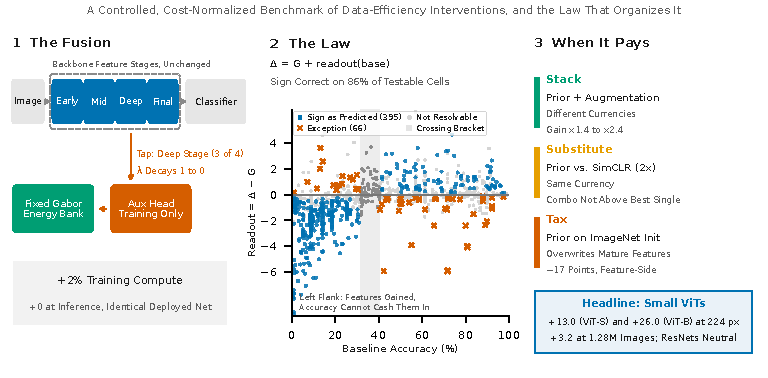
\includegraphics[width=0.98\columnwidth]{figs/graphical_abstract.pdf}
\end{graphicalabstract}
\fi

\ifsubmissionmode\else
\begin{highlights}
\item A \computeCells-configuration benchmark of data-efficiency interventions
\item Splitting one instrument's bands pays; pairing two satellites does not
\item A measurable rule predicts stacking, substitution or interference
\item Free prior beats 2$\times$-compute SSL on small ViTs; at 5$\times$ the ordering flips with data
\item Attention's feature deficit persists at 1.28M images and grows with scale
\end{highlights}
\fi

\begin{keywords}
information fusion \sep data-efficient learning \sep hand-crafted priors \sep
self-supervised learning \sep auxiliary losses \sep benchmark
\end{keywords}

\maketitle
\sloppy  % CAS columns are narrow; prefer loose spacing over margin overrun

%% ------------------------------------------------------------------
%% ---------------------------------------------------------------------
\section{Introduction}\label{sec:intro}

A bank of Gabor filters, fixed before training and free to compute, is worth
$+26$ accuracy points to a ViT-B/16 at $224$\,px. Injected exactly the same way
into a network that has already had contrastive pre-training, it is worth
nothing. Injected at the same strength into one initialized from ImageNet, it
costs $15$ to $17$ points. One
intervention, one frozen recipe, one code path: three outcomes spanning more
than forty accuracy points. The useful question is not which number is representative,
because none of them is. It is what distinguishes the three cases, and whether
that can be determined \emph{before} the combination is trained.

This is the general situation, not a curiosity of one prior. Every practitioner
who has trained a network on a small dataset faces the same menu of remedies:
pre-train on ImageNet \citep{he2019rethinking}, run a self-supervised stage
\citep{chen2020simclr,caron2021dino}, augment more aggressively
\citep{touvron2021deit}, or inject prior knowledge into the model
\citep{vonrueden2023informed}. Each fuses an external source of
information (weights learned elsewhere, invariances distilled from augmented
views, hand-crafted structure) with whatever the labeled data can teach on its
own. What the field lacks is not remedies but a controlled account of how these
sources \emph{combine}: when does adding a second source help, when is it
redundant with what the first already supplies, and when does the fusion
actively destroy value? These three outcomes, which we call \emph{stack},
\emph{substitute} and \emph{interfere}, are usually discovered anecdotally, one
paper and one setting at a time, under training recipes that differ in a dozen
uncontrolled ways.

Our answer is that sources trade in identifiable \emph{currencies}, and that
what a source is worth depends on which currency is scarce; how modern the
method is matters far less. Two sources add only when their currencies differ,
a necessary condition: whether the possible gain is realized also depends on
the architecture and on the strength at which the second source is applied.
This is not a metaphor we impose after the fact: each source's currency is
measurable, on frozen features, from each source \emph{alone}. That is what
lets the three outcomes above be anticipated from quantities measurable before
the combination is trained, and it is why the same free prior can be the most
valuable intervention we measure in one setting and the most damaging in
another.

This paper treats the question as a measurement problem. We build a single
instrument (one frozen training recipe, fixed data subsets shared by every run,
and a numerically pinned bank of Gabor and moment spectral filters
\citep{luan2018gaborcnn,bruna2013scattering}) and use it
to measure one deliberately austere source of prior knowledge against
representative data-driven alternatives at matched or declared compute. The
prior, which we call \emph{MomentAux}, could hardly cost less: a fixed bank of
oriented-energy targets, injected only during training through a small
auxiliary regression head whose loss weight decays to exactly zero, costing
${\sim}2\%$ extra training compute and \emph{nothing} at inference. Against it
we field SimCLR \citep{chen2020simclr}, SimSiam \citep{chen2021simsiam} and
DINO \citep{caron2021dino} initializations (each ${\sim}2\times$
compute), ImageNet transfer \citep{he2019rethinking}, DeiT-strength
augmentation \citep{touvron2021deit}, learned FitNets-style
teachers \citep{romero2015fitnets}, and targets built from histograms of
oriented gradients (HOG) \citep{dalal2005hog}. The
resulting grid spans 13 datasets across six visual domains, nine backbone
families from ResNet-18 \citep{he2016resnet} to ViT-B/16
\citep{dosovitskiy2021vit}, data scales from 150 to 1.28M images,
resolutions from $32$ to $224$\,px, and \computeCells{} configurations trained
over \computeRuns{} runs, each with a retained run record.

A grid of this size threatens to be a table dump. What rescues it is an
empirical law we found, not assumed, and then tested by registering its
predictions in advance and trying to break them. Writing $\Delta$ for an
intervention's end-to-end accuracy gain and $G$ for the gain a linear
evaluation \citep{alain2016understanding} reads from its frozen features under
identical probing, we find across the grid that
\begin{equation}
  \Delta \;=\; G \;+\; \readout(\mathrm{base}),
  \label{eq:law}
\end{equation}
Run the evaluation at a practitioner's own label budget and $G$ predicts
$\Delta$ to $0.17$ points across 30 cells and seven datasets, which values a
combination without training it; the sign law below is its full-label
corollary, resting on far more cells (Sec.~\ref{sec:law}). Under that fixed
protocol the \readout{} term depends, to a good approximation, only on the
\emph{baseline accuracy} of the cell: negative below a crossing at
${\sim}32$--$40\%$ accuracy, near zero at the crossing, and small and positive
above it. The sign holds in $\auditRate\%$ of the \auditResolvable{} cells
where measurement uncertainty allows it to be tested and in $\auditBelowRate\%$ of those
below the crossing, and its quantitative form survived our hardest
pre-registered tests: it predicted the feature gain of a backbone family it had
never seen (Swin) from baseline heights alone, and at ImageNet scale it tied
end-to-end gains to feature gains within $1.1$ accuracy points on five of six
backbone pairs (Sec.~\ref{sec:scale}).

The law converts the grid into an explanation, and it is where currency stops
being a metaphor and becomes the term $G$: heavy augmentation supplies
nuisance-invariance, contrastive pre-training much the same invariance at
greater expense, ImageNet weights mature photographic features, and the moment
prior oriented-energy structure. Same-currency fusions substitute: the prior
and SimCLR each render the other nearly worthless, and their combination never
beats the better single. Different-currency fusions can stack, the prior's gain
growing $1.4$--$2.4\times$ under DeiT-strength augmentation on the attention
backbones, though on two convolutional populations off the selection set the
same pairing stacks
at one cell of six: differing currencies are necessary, not always
sufficient. And fusing a shaping prior at full strength into an
initialization that already carries mature features interferes in
proportion to what the initialization supplied, a cost that lands almost
entirely on the features themselves and that a weaker
auxiliary weight removes (Sec.~\ref{sec:fusion}).

Two headline findings illustrate what the instrument can resolve. First, small
vision transformers carry a large feature deficit that the prior fills: the
gain reaches $+13.0$ points for ViT-S/16 and $+26.0$ for ViT-B/16 on
ImageNet-100 at $224$\,px under the standard DeiT recipe at a shared
$100$-epoch budget, and persists at $+3.2$ after 1.28 million images where the
ResNet baseline is exactly neutral ($+0.04$). The budget is part of that claim,
so we doubled it on both models: the gains become $+4.52 \pm 0.18$ for ViT-S
and $+6.71 \pm 0.90$ for ViT-B, a quarter to a third of the headline figures but
\emph{growing} with model scale still, at $2.4$ standard errors
(Sec.~\ref{sec:scale}). Second, the fashionable remedy is
not
always the right one: under plain augmentation SimCLR beats the prior across
the mid-data band on photographic datasets, but under the DeiT recipe the
comparison flips at matched ${\sim}2\times$ cost, at every CIFAR-100 fraction
and at all but a statistical tie at Tiny-ImageNet's largest, because the
recipe supplies the invariance SimCLR was paid that compute to learn. At
$5\times$ the flip narrows to the higher-data band, where the prior still wins
on both populations, while the comparator takes the scarcest cells
(Sec.~\ref{sec:budget}); the ordering tracks the data fraction, a
statement about budget and regime, not a ranking of methods.

\paragraph{Contributions.}
\begin{enumerate}
  \item \textbf{An instrument, not just experiments} (Sec.~\ref{sec:instrument}):
    a frozen recipe with fixed subsets, pinned filter banks, declared
    cost normalization, and pre-registered predictions with falsifiers,
    every headline table regenerable from the released artifacts.
  \item \textbf{The grid} (Sec.~\ref{sec:grid}): $\computeCells$ configurations,
  $\computeRuns$ runs,
    comparing a free spectral prior against SSL, transfer, augmentation and
    learned teachers across 13 datasets, 9 backbones and
    150 to 1.28M images.
  \item \textbf{The law, led by its budget-matched form}
    (Sec.~\ref{sec:law}): at a practitioner's own label budget the
    frozen-feature gain predicts the end-to-end gain to $0.17$ points over 30
    cells and seven datasets, which values an intervention without training
    it. The full-label sign law of $\Delta = G +
    \readout(\mathrm{base})$ is its explanatory corollary, validated from
    CIFAR scale to ImageNet scale, with its boundary cases reported as
    findings, including the one patterned failure where features improve at
    sufficiency while accuracy does not follow (Sec.~\ref{sec:exceptions})
    and the ImageNet-scale puzzle of three envelope shapes on identical data
    (Sec.~\ref{sec:scaleenvelope}).
  \item \textbf{A fusion taxonomy with mechanism}
    (Sec.~\ref{sec:fusion}): stack, substitute, or interfere, decided by
    whether the fused sources carry the same information currency, with the
    interference conditioned on shaping strength, and
    verified on the feature side, not just end-to-end.
  \item \textbf{A procedure, not only a taxonomy}
    (Sec.~\ref{sec:procedure}): because each source's currency is
    measurable from that source \emph{alone}, the outcome of combining two
    follows from quantities measurable before the combination is trained. We
    state this as an
    algorithm, run it end to end on a pair whose answer we then verify by
    training, marking that run illustrative, not prospective, for a
    protocol reason we give there, and distil the grid into a regime-indexed
    guide with costs attached (Sec.~\ref{sec:guide}).
\end{enumerate}

%% ---------------------------------------------------------------------
\section{Related work}\label{sec:related}

\looseness=-1 We group prior work by the mechanism through which it supplies
information to a data-limited network, since that is the axis along which our
comparison is organized: hand-crafted structure placed in the forward path;
auxiliary and distillation targets that shape features during training;
self-supervised and transfer initializations that pay compute for
representation; augmentation recipes that supply invariance; small-data results
specific to attention; and the large-scale comparative benchmarks that most
closely resemble what we build. Section~\ref{sec:fusiontheory} then places our
three outcomes against the
fusion literature's own account of how sources relate, and
Sec.~\ref{sec:gap} states, in a single table, which properties a controlled
fusion study requires and which of them each line of work currently provides.

\paragraph{Hand-crafted structure inside learned networks.} Fixed oriented
filters predate deep learning as image descriptors \citep{dalal2005hog}.
Scattering networks showed that cascades of fixed wavelets rival learned
features in small-data regimes \citep{bruna2013scattering}, and
Gabor-structured convolutions have been used to regularize or cheapen early
layers \citep{luan2018gaborcnn}. These lines place the structure \emph{in the
forward path}, where it occupies input bandwidth permanently. Our forward-path
baselines reproduce their known failure mode, a mid-data penalty band that no
filter choice escapes (Sec.~\ref{sec:ablations}), and our central object
differs precisely in that the structure lives in a training-only auxiliary
target whose influence decays to zero, so abundant data can override the prior
instead of paying for it.

\paragraph{Auxiliary targets, deep supervision, and distillation.}
\looseness=-1 Regressing intermediate features onto targets is the mechanism of
FitNets \citep{romero2015fitnets} and deep supervision \citep{lee2015deeply};
HOG targets power MaskFeat's self-supervised pre-training
\citep{wei2022maskfeat}. What distinguishes our setting is the \emph{fixedness
and cost} of the target: no teacher network is trained, no pre-training stage
is run, and the target is a closed-form function of the input. Our controls
quantify how much this matters: a learned same-data teacher moves accuracy by
at most $0.73$ points anywhere on an eleven-point envelope, HOG targets
recover a third to a half, and a random fixed target of identical shape is
beaten by $+0.8$ to $+4.2$ points on all four populations where we ran
that control (Table~\ref{tab:controls}, Sec.~\ref{abl:target}), so the
gain traces to the moment structure itself, not to auxiliary
regression as a mechanism.

\paragraph{Self-supervised learning (SSL) as initialization.} Contrastive and
self-distilling pre-training
\citep{chen2020simclr,chen2021simsiam,caron2021dino} is the modern default
source of ``free'' features. \citet{ericsson2022why} measure \emph{which}
invariances such models learn and show that fusing representations with
complementary invariances improves transfer, which is close in spirit to our
different-currency case; the difference is that they demonstrate the
complementarity, while we attempt a prospective, cost-normalized decision rule
for complementarity, redundancy and interference. Much less is measured about
the small-data,
from-scratch regime we target, and each of those methods is evaluated here
under its own published recipe for this scale. Our
grid contributes three facts to that gap: negative-free SimSiam learns
essentially nothing at $2.5$--$25$k images under its published CIFAR recipe,
though four times that budget recovers up to $+4.3$ and we report it as a
property of the budget, not of the method; SimCLR is strong on
photographic statistics but loses to a free domain-agnostic prior on satellite
imagery in the low-data band; and the SSL-versus-prior comparison inverts under
a modern supervised recipe at matched cost, because the augmentation stack
substitutes for the invariance SSL sells (Secs.~\ref{sec:fusion} and
\ref{sec:budget}).

\paragraph{Transfer learning.} ImageNet initialization remains the strongest
single intervention on photo-like data, with known limitations under domain
shift and with training-from-scratch competitive given enough data
\citep{he2019rethinking}. We use transfer both as a comparator and as a test of
fusion: injecting the spectral prior at full auxiliary strength \emph{on top
of} ImageNet weights is the
one configuration in our grid that is destructive everywhere, and linear
probing shows the destruction is feature-side, early shaping erasing the
mature structure the initialization supplied, in proportion to how much that
structure was worth (Sec.~\ref{sec:fusion}).

\paragraph{Small-data vision transformers.} That ViTs underperform without
large data or heavy regularization is well documented
\citep{dosovitskiy2021vit,touvron2021deit}, and a family of remedies exists:
distillation tokens \citep{touvron2021deit}; architectures that reintroduce the
hierarchical, local inductive bias attention lacks, such as Swin
\citep{liu2021swin}, which we include as a backbone for that reason; and
auxiliary self-supervised objectives trained jointly with the classifier, of
which \citet{liu2021efficientvit} is the closest antecedent to this work: a
dense relative-localization task added for exactly this deficit, differing from
ours in that its target is computed from the images themselves, where ours is
pinned in advance. Our contribution to this literature is quantitative and
comparative: we measure the deficit as a feature quantity ($G \approx 13$--$15$
points for ViT-tiny across $2.5$--$12.5$k images, roughly $2.3\times$ the
ResNet-18 value at matched cells), show a fixed spectral target fills it at lower cost
than contrastive pre-training and more effectively than DeiT augmentation
alone, and show the deficit \emph{grows} with model scale at full data
(Sec.~\ref{sec:scale}), which argues it reflects data-hunger, not
small-model capacity.

\paragraph{Large-scale comparative benchmarks.} Two recent efforts share our
comparative ambition and clarify what is still missing. \emph{Battle of the
Backbones} \citep{goldblum2023battle} compares a broad suite of pretrained
backbones across tasks over more than 1{,}500 training runs, and finds
supervised convolutional pre-training still competitive with self-supervised
and vision-language alternatives. \citet{marks2025closer} take a closer look at
self-supervised benchmarking specifically, and show that conclusions depend
heavily on the evaluation protocol chosen. Both benchmark \emph{pretrained
backbones}, so their unit of comparison is a checkpoint someone else produced,
and neither normalizes by training cost nor asks what happens when two sources
of information are combined. Our unit is instead the \emph{intervention applied
to a fixed recipe}, which is what makes cost normalization and the stacking
question answerable.

\paragraph{Spectral structure inside transformers.} A parallel line injects
spectral structure into attention architectures: FViT \citep{shi2026fvit} adds
a \emph{learnable} Gabor filter to focus attention across scales and
orientations, and scattering-based token mixers do the same with wavelet
decompositions. These are architectural changes that persist at inference, and
each is evaluated as a model proposal against published baselines. Our object
is the complement: the filters are fixed, not learned, they never enter
the forward path, and the deployed network is unchanged, which is what lets us
ask the benchmark question of when adding them pays instead of the model
question of whether one architecture beats another.


\subsection{Relation to fusion theory}\label{sec:fusiontheory}
The outcomes we measure are not new categories, and we set out the prior claims
before our own. \citet{durrantwhyte1988sensor} classified the interactions
between disparate information sources as \emph{cooperative}, \emph{competitive}
and \emph{complementary}; the surveyed form now standard in the field
\citep{khaleghi2013multisensor} states the triple as complementary, redundant
and cooperative, where complementary sources describe different aspects of the
target, redundant sources describe the same aspect, and cooperative sources
jointly yield what neither yields alone. Our \emph{stack} is complementary
combination and our \emph{substitute} is redundant combination. We adopt that
vocabulary here and use our own terms only as informal labels for it.

\citet{dasarathy2001what} organizes the field's questions as what, where, why,
when and how to fuse, and observes that the \emph{when} has received least
attention because it is the one that cannot be answered from the architecture.
That is the question this paper takes up, in the specific setting where one
source is hand-crafted and the other is learned from the data. Knowledge
fusion itself is likewise an established object of study
\citep{khaleghi2013multisensor}: \citet{smirnov2019knowledge} surveys the
patterns
by which knowledge and data are combined, and catalogs the same three outcomes
we recover. What that survey records as patterns to be chosen by a designer, we
measure as outcomes to be predicted from the sources, which is the difference
between a taxonomy and a decision procedure. The field's benchmarks have
generally compared \emph{algorithms} for a fixed fusion problem; ours compares
\emph{sources} under a fixed algorithm, holding the recipe frozen so that what
varies is the knowledge injected, not the method injecting it.

One difference is substantive, not terminological, and it sharpens what a
representation-learning setting adds. In sensor fusion redundancy is a
\emph{virtue}: two instruments measuring the same quantity reduce variance and
buy fault tolerance. In ours it is waste, because performance is bounded by the
information the sources share, and supplying that information twice improves
nothing.
Redundancy pays for reliability and not for representation quality, and a
taxonomy built for the first case does not transfer its sign to the second.

Our third outcome, in which a source destroys what its partner supplied, is
likewise not new, and has at least three names: \emph{catastrophic fusion}
\citep{movellan1997catastrophic}, negative transfer \citep{wang2019negative},
and the modality competition of \citet{wang2020multimodal}, who report
that the best unimodal network often beats the jointly trained multimodal one
despite the latter receiving strictly more information. What we add is not the
phenomenon but its magnitude law: the damage scales with how much the displaced
source had contributed, and vanishes exactly where it had contributed nothing.

The formal account of our informal ``currency'' is partial information
decomposition \citep{williams2010nonnegative}, which splits what two sources
tell us about a target into unique, redundant and synergistic atoms, and which
\citet{liang2023quantifying} have already carried into deep multimodal learning
with estimators that scale and with a-priori model selection as the
application. We do not compute it. Our measurement is a linear-evaluation gap
on frozen features: inexpensive enough for \computeCells{} cells, ordinal, not
an information quantity, and blind to anything not linearly decodable. Read our
result as an empirical instance of the decomposition those authors formalize,
not as an estimate of it.

Two further connections position the predictor, not the taxonomy. Predicting a
downstream outcome from an inexpensive measurement, without training the
combined system, is the programme of transferability estimation
\citep{nguyen2020leep}, which scores a single pre-trained source; ours asks the
same question of a \emph{pair}. And the challenge that programme raises for us
is direct: \citet{newell2020useful} report that linear evaluation does not
correlate with fine-tuning performance in general. Our defence is narrow and
empirical, not a rebuttal. We do not use the linear evaluation to rank absolute
quality; we use the \emph{gap} between two arms probed under an identical
protocol, on checkpoints that differ in one intervention, and we report how
well that gap predicts the paired difference (Sec.~\ref{sec:law}) rather
than assuming it does.

Finally, our knowledge source sits where \citet{vonrueden2023informed} make
precise. Their taxonomy classifies informed learning by knowledge
\emph{source}, \emph{representation} and \emph{integration point}, and states
that informed learning requires two independent sources of information, data
and prior knowledge, which is the reading of ``two sources'' under which this
study is a fusion study. Ours is scientific knowledge about early vision,
represented as a pinned filter bank, integrated at the learning algorithm; the
nearest existing method is their own informed pre-training, which condenses
knowledge into prototypes for initialization where ours enters as a decaying
auxiliary target. That survey catalogs where knowledge can be injected; what it
does not settle, and what a practitioner must decide, is \emph{when} injecting
it is worth anything given what the data and the available pre-trained
artifacts already supply. That is the question this benchmark answers, and we
claim only that: we found no controlled,
compute-declared answer to it, not that no neighbouring question has been
answered.

\subsection{The gap this paper closes}\label{sec:gap}

\begin{table}[pos=htbp]
\caption{Where the literature stands on the five properties a fusion
question needs, and what this work adds. \cmark{} = property present;
\pmark{} = partial or incidental; \xmark{} = absent. ``Cost-normalized''
means comparators are reported against a declared training-compute
multiple, not each method's own chosen budget;
``feature-side'' means the effect is measured on frozen representations,
not only end-to-end; ``combination'' means the study measures what
happens when two sources are applied together.}
\label{tab:gap}
\centering\scriptsize
\setlength{\tabcolsep}{2.6pt}
\zebra{2}
\begin{tabular}{lccccc}
\toprule
Line of work & \rotbox{one frozen recipe} & \rotbox{cost-normalized} &
  \rotbox{feature-side} & \rotbox{combinations} & \rotbox{predictive model} \\
\midrule
Fixed spectral filters in the forward path
  \citep{bruna2013scattering,luan2018gaborcnn,shi2026fvit}
  & \pmark & \xmark & \xmark & \xmark & \xmark \\
Auxiliary and distillation targets
  \citep{romero2015fitnets,lee2015deeply,wei2022maskfeat}
  & \pmark & \xmark & \pmark & \xmark & \xmark \\
Self-supervised pre-training
  \citep{chen2020simclr,chen2021simsiam,caron2021dino}
  & \xmark & \xmark & \cmark & \xmark & \xmark \\
Transfer learning studies
  \citep{he2019rethinking}
  & \pmark & \xmark & \pmark & \xmark & \xmark \\
Small-data ViT recipes
  \citep{touvron2021deit}
  & \xmark & \pmark & \xmark & \pmark & \xmark \\
Backbone and self-supervised benchmarks
  \citep{goldblum2023battle,marks2025closer}
  & \pmark & \xmark & \cmark & \xmark & \xmark \\
Classical fusion taxonomy
  \citep{durrantwhyte1988sensor,williams2010nonnegative}
  & \xmark & \xmark & \xmark & \cmark & \pmark \\
\midrule
\textbf{This work} & \cmark & \cmark & \cmark & \cmark & \cmark \\
\bottomrule
\end{tabular}
\end{table}

Table~\ref{tab:gap} summarizes the position. Each column is a property that a
question about \emph{fusing} information sources requires, and no existing line
supplies all five at once.

The first column matters because comparisons made under each method's own
preferred recipe cannot attribute a difference to the method; the backbone
benchmarks above inherit whatever recipe produced each checkpoint. We instead
hold one recipe and one set of fixed image indices and vary only the
intervention.

The second is rarely reported: self-supervised pre-training roughly doubles
the training compute of the baseline it improves, yet that factor almost never
appears beside the accuracy it buys, leaving ``method A beats method B''
unanswerable at a fixed budget. Every comparator here carries a declared
multiple.

The third and fourth columns are what turn a table of numbers into an
explanation. Linear probing is standard practice for evaluating self-supervised
representations, so the feature-side view exists in that literature; what is
missing is applying it to a \emph{paired} comparison, the same intervention
measured end-to-end and on frozen features at once, which is what exposes
redundancy between two sources. Combinations are the least studied of all:
what happens when a prior is applied on top of augmentation, of
self-supervised weights, or of a pretrained initialization is
precisely the fusion question, and we could find no controlled study that
measures all three.

The fifth column is the one we regard as the paper's distinguishing
contribution. Benchmarks describe; a law predicts. Our decomposition $\Delta =
G + \readout(\mathrm{base})$ was registered in advance and used to call
all three classes of unmeasured quantity listed above before those measurements
existed (Secs.~\ref{sec:law} and~\ref{sec:scale}). A related decomposition
of learning dynamics into representation and decoding components has been
proposed for grokking \citep{liu2022grokking}; to our knowledge no comparable
predictive account exists for data-efficiency interventions.

%% ---------------------------------------------------------------------
\section{The instrument}\label{sec:instrument}

The benchmark's claims rest on the comparisons being controlled, so we
describe the controls before the results.

\subsection{Frozen recipe and committed subsets}
Every headline cell trains with an identical recipe: SGD with momentum
$0.9$, learning rate $0.1$, weight decay $5{\times}10^{-4}$, cosine
schedule, 200 epochs, batch size 128, and random-crop + horizontal-flip
augmentation only. The recipe is frozen in the strict sense: no cell tunes
it, and any configuration that must deviate (AdamW for architectures the
SGD recipe cannot train, reduced epochs at ImageNet scale, added
augmentation stacks) carries a diagnostic namespace and never enters a
headline table; within such cells both arms of every comparison share the
deviation, so paired differences remain valid.

Data fractions are not sampled at run time. For every dataset and fraction
we commit stratified subset indices to version control, so every
intervention -- baseline, prior, SSL initialisation, transfer -- sees
byte-identical images. Even the dataloader worker count is part of the
reproducibility contract, because PyTorch seeds per-worker augmentation
streams: we verified that changing it re-draws augmentations (validly but
non-reproducibly) and therefore pin it per cell.

\subsection{The prior: MomentAux}
The knowledge source under test is a bank of eight complex Gabor
quadrature pairs (two spatial scales, four orientations) whose
phase-invariant magnitude responses form an oriented-energy map of the
input -- the classical spectral description of early vision
\citep{jones1987gabor}. The bank is \emph{pinned}: unit tests fingerprint
its numerical values, so no result can drift with a library version.

During training only, a $1{\times}1$ convolutional head taps the
backbone's third stage and regresses (MSE) onto the bank's magnitude maps,
weighted by $\lambda$ that follows a cosine schedule from $\lambda_0$
to exactly zero. Because $\lambda$ reaches zero, late training is pure
cross-entropy; high-data neutrality is structural rather than tuned. The
deployed network is byte-identical to the baseline: same FLOPs, same
parameters, no extra inference cost. Training overhead is ${\sim}2\%$.
One setting -- $\lambda_0{=}1.0$, magnitude target, third-stage tap, with
head-norm projection (Section~\ref{sec:ablations}) -- transplants across
every dataset and backbone in the study without retuning; we call it the
\emph{champion} configuration and use it verbatim unless stated.

\subsection{Comparators and cost normalisation}
We normalise by declared training cost relative to the baseline:
MomentAux ${\approx}1.02\times$; SimCLR, SimSiam and DINO initialisations
$2\times$ (a full pre-training stage on the same subset images, then the
frozen recipe); ImageNet transfer (amortised, but an external-data
advantage we flag); DeiT-strength augmentation \citep{touvron2021deit}
${\approx}1\times$ compute but a modern recipe change; FitNets teachers
$2\times$; HOG targets ${\approx}1.02\times$. SSL pre-training uses each
method's published small-image protocol, and we additionally verify SimCLR
was given its best shot: strengthening its views to DeiT strength
\emph{hurts} it at every fraction tested (Section~\ref{sec:fusion}).

\subsection{Measuring features: the probe protocol}
The law needs a feature-side quantity. For every trained pair we fit a
multinomial logistic probe (LBFGS, fixed hyper-parameters) on frozen
penultimate features over the full training split, and define $G$ as the
aux-minus-baseline probe gap under identical probing
\citep{alain2016understanding}. Probes are diagnostics, never headline
numbers. Two scope rules, learned during the study and enforced
throughout: a probe is trustworthy only while it holds substantially more
labels than the cell trained on (at 100\% cells the $G$/readout split is
not interpreted); and at ImageNet64 scale, where a 1.28M-row LBFGS is
impractical, probes use fixed per-class budgets that are compared only
within the same budget.

\subsection{Pre-registration}
Each experimental wave was launched with numeric prediction bands and
explicit falsifiers recorded in the project ledger before any result
existed. We report outcomes against those bands, including the misses:
of the major predictions in this program, several failed in instructive
ways (our ``SSL is data-regime-bounded'' prediction was wrong; our
``augmentation substitutes for the prior'' prediction was wrong in the
opposite direction), and both failures became findings
(Section~\ref{sec:fusion}). Seed counts are three per cell minimum, ten
for headline envelopes; cells with collapsed seeds are flagged bistable
and excluded from headline status as a finding in their own right.

%% ---------------------------------------------------------------------
\section{The grid}\label{sec:grid}

\begin{table}[t]
\caption{The benchmark at a glance. Every cell trains the frozen recipe of
Section~\ref{sec:instrument}; costs are declared multiples of baseline
training compute.}
\label{tab:glance}
\centering\small
\begin{tabular}{@{}ll@{}}
\toprule
\textbf{Axis} & \textbf{Coverage} \\
\midrule
Datasets (14+2) & CIFAR-10/100, ciFAIR-100, STL-10, Tiny-ImageNet,\\
 & coarse/relabelled variants; EuroSAT, DTD, Food-101,\\
 & PathMNIST, CUB-200; ImageNet64, ImageNet-100 \\
Domains & photographic, satellite, texture, food, histopathology \\
Backbones (7) & ResNet-18/34/50, MobileNetV3, ConvNeXt-T, \\
 & ViT (tiny/S/B), Swin-T \\
Data scale & 500 $\rightarrow$ 1.28M images; 10 $\rightarrow$ 1000 classes \\
Resolution & 32, 64, 96, 224\,px \\
Interventions & MomentAux (${\sim}1.02\times$); SimCLR/SimSiam/DINO \\
 & ($2\times$); ImageNet transfer; DeiT augmentation; \\
 & FitNets teacher ($2\times$); HOG target; combinations \\
Measured cells & ${\sim}7{,}500$ (${\geq}3$ seeds; envelopes at 10) \\
\bottomrule
\end{tabular}
\end{table}

Table~\ref{tab:glance} summarises the design space. Three views of the
grid organise the results that follow.

\subsection{The prior's own envelope}
\begin{table}[t]
\caption{End-to-end gain $\Delta$ of the champion prior over the shared
baseline (percentage points, mean $\pm$ SEM of the difference). Ten seeds
per arm on bold cells, three elsewhere. The envelope is unimodal in the
data fraction on every dataset; at 100\% the prior is neutral by
construction ($\lambda \to 0$).}
\label{tab:envelope}
\centering\small
\setlength{\tabcolsep}{4.2pt}
\begin{tabular}{@{}lrrrrrrrr@{}}
\toprule
 & \multicolumn{8}{c}{\textbf{data fraction}} \\
\cmidrule(l){2-9}
\textbf{dataset} & 1\% & 2\% & 5\% & 10\% & 15\% & 25\% & 50\% & 100\% \\
\midrule
CIFAR-100 & $\mathbf{+1.42}$ & $+2.50$ & $\mathbf{+5.15}$ & $\mathbf{+3.75}$ & $+2.55$ & $+0.25$ & -- & $+0.08$ \\
CIFAR-10 & $\mathbf{+6.37}$ & $\mathbf{+6.66}$ & $+4.41$ & $+1.09$ & $-0.66$ & $-0.83$ & -- & $-0.26$ \\
Tiny-ImageNet & $+1.49$ & $+1.81$ & $\mathbf{+2.12}$ & $+1.65$ & -- & $+0.10$ & -- & $-0.42$ \\
STL-10 & -- & -- & -- & $+5.92$ & -- & -- & $+3.18$ & -- \\
EuroSAT & $+2.67$ & $+1.60$ & $+0.84$ & $+1.22$ & $+0.16$ & ${\sim}0$ & ${\sim}0$ & ${\sim}0$ \\
Food-101 & -- & -- & $+5.63$ & $+3.18$ & $+0.46$ & -- & $-0.47^{\dagger}$ & $-0.47$ \\
DTD & -- & -- & $+0.30$ & -- & $+2.15$ & -- & -- & $+3.55$ \\
PathMNIST & $+5.7$ & -- & -- & $+1.74$ & -- & $-0.5^{\ddagger}$ & -- & $-$ \\
CUB-200 & \multicolumn{6}{c}{\small (deep left flank; $+0.56$ at 25\%)} & & $+2.74$ \\
\bottomrule
\multicolumn{9}{@{}p{0.94\linewidth}@{}}{\footnotesize $^{\dagger}$50\%
shown in the 100\% column position for Food-101 where measured.
$^{\ddagger}$PathMNIST cells above ${\sim}15\%$ are confounded by a
distribution-shifted test split that penalises \emph{all} methods
(Appendix~\ref{app:domains}); we treat only its low-data cells as
interpretable.} \\
\end{tabular}
\end{table}

Table~\ref{tab:envelope} shows the prior's gain over the baseline across
the data axis. Three regularities recur. The envelope is
\emph{unimodal}: gains rise from the extreme-scarcity floor, peak in a
dataset-specific band, and decay toward zero as data becomes sufficient.
The peak's location tracks the dataset's difficulty rather than its
fraction -- easy ten-way CIFAR-10 peaks by 1--2\% and is already negative
at 15\%, while hundred-way CIFAR-100 peaks at 5\%. And at full data the
prior is neutral within noise on every one of ten populations, which is
what the $\lambda \to 0$ schedule is for: the fusion asks nothing when the
data can pay for everything.

\subsection{The multi-method comparison}
The same envelope measured for every comparator produces the head-to-head
tables that Sections~\ref{sec:fusion} and \ref{sec:guide} analyse. As a
preview of their shape: on CIFAR-100 under plain augmentation, SimCLR
initialisation at $2\times$ compute beats the $1.02\times$ prior by
$+0.85$ to $+5.0$ points between 1\% and 10\% and converges back to parity
by 50\%; SimSiam learns nothing at this scale (${\leq}+0.9$ everywhere);
DINO trails the prior at every fraction below 25\%. On attention
backbones, and on any backbone under a modern augmentation recipe, the
ordering inverts (Section~\ref{sec:fusion}).

\subsection{Attention: the regime where the prior is dramatic}
\begin{table}[t]
\caption{ViT-tiny on CIFAR-100: gain of the prior under the plain recipe
($\Delta_{\mathrm{plain}}$) and under DeiT-strength augmentation
($\Delta_{\mathrm{DeiT}}$), and the amplification ratio. Augmentation does
not substitute for the prior; it amplifies it and shifts its peak toward
more data. Three seeds per cell.}
\label{tab:vitenvelope}
\centering\small
\setlength{\tabcolsep}{4.5pt}
\begin{tabular}{@{}lrrrrrrrrr@{}}
\toprule
fraction & 1\% & 2\% & 3\% & 5\% & 7\% & 10\% & 15\% & 25\% & 100\% \\
\midrule
$\Delta_{\mathrm{plain}}$ & $+1.4$ & $+3.3$ & $+6.2$ & $+9.4$ & $+11.0$ & $+13.3$ & $\mathbf{+14.4}$ & $+13.7$ & $+9.9$ \\
$\Delta_{\mathrm{DeiT}}$ & $+3.2$ & $+6.0$ & $+9.5$ & $+16.3$ & $+18.7$ & $+21.0$ & $+24.6$ & $\mathbf{+25.1}$ & $+13.9$ \\
ratio & 2.2 & 1.8 & 1.5 & 1.7 & 1.7 & 1.6 & 1.7 & 1.8 & 1.4 \\
\bottomrule
\end{tabular}
\end{table}

Table~\ref{tab:vitenvelope} previews the study's most striking axis.
ViT-tiny trained from scratch gains $+9.9$ points from the prior even at
\emph{full} CIFAR-100 -- a scale at which every convolutional backbone is
neutral -- and under the standard DeiT recipe the gains grow to
$+25$ points, peaking later in the data axis. The best ViT number in the
study, $75.3\%$ at full CIFAR-100, is DeiT augmentation \emph{plus} the
prior, against $61.4\%$ for the recipe alone. Sections~\ref{sec:law} and
\ref{sec:scale} show this is a feature-side phenomenon that persists to
ImageNet scale and grows with model size.

%% ---------------------------------------------------------------------
\section{The organizing law}\label{sec:law}

\looseness=-1 A grid of $\computeCells$ cells is only as useful as the account that organizes
it. The practical headline of this section is its budget-matched result:
evaluated at a cell's own label budget, the frozen-feature gain predicts the
end-to-end gain to $0.17$ points on average over 30 cells and seven datasets
(end of Sec.~\ref{sec:lawaudit}), so an intervention can be valued without
training it. The full-label sign law is the explanatory account behind that
result, and the rest of the section is built around it. We state its form, in
which the end-to-end gain $\Delta$
decomposes into a feature term $G$ and a \readout{} term governed by baseline
accuracy, and what the law is not (Sec.~\ref{sec:lawform}); audit that
form over the whole grid under a resolvability criterion that keeps
uninformative cells from inflating the score (Sec.~\ref{sec:lawaudit});
give the three episodes that distinguish a law from a curve fit, calling
unmeasured quantities in advance including for a backbone family it had never
seen (Sec.~\ref{sec:lawpredict}); and localize what each term depends on,
which is what makes the fusion outcomes of Sec.~\ref{sec:fusion}
anticipatable, not merely observed (Sec.~\ref{sec:lawG}).

\subsection{Form and origin}\label{sec:lawform}
For each paired cell we measure the end-to-end gain $\Delta$ and the feature
gain $G$ (Sec.~\ref{sec:instrument}), and define $\readout \equiv
\Delta - G$.

\textbf{What is definitional and what is not.} Eq.~\ref{eq:law} is true by
construction, and we state that plainly: $\Delta = G + (\Delta - G)$
decomposes a measured quantity and cannot fail. It earns its place by naming
two terms that behave and are measured differently, not by
being a discovery. \emph{Every} empirical claim we make lives in the second
term: that its \textbf{sign} is predictable from baseline accuracy alone,
before the cell is trained. Where we write ``the law'' below we mean that sign
regularity, never the identity. What that sign \emph{means} depends on the
evaluation's label budget, which we measure instead of assuming at the end of
Sec.~\ref{sec:lawaudit}.

\looseness=-1 Across the grid, baseline accuracy is the largest single determinant of this
term and the only one whose effect is consistent in sign across datasets and
backbones. We are deliberate about how strong that claim is: binned on baseline
accuracy alone the \readout{} term has $R^2 = 0.27$, dataset identity explains a
further $0.13$ of the residual, data fraction $0.02$ and backbone essentially
none ($0.003$), and the
residual standard deviation at fixed baseline is $\auditResidSD$ points. This
is a first-order trend with substantial scatter, not a curve that pins a cell's
\readout{}. All five moved with the scope repairs of Sec.~\ref{sec:lawaudit},
chiefly the first, since
the cells that repair removed carry large negative $\Delta$ and $G$ and were the
widest-scattered points in the fit. What is robust is the \emph{sign}, which is
what this section audits. The term is strongly negative at low baselines, where
features improve more than accuracy can show because a classifier with five
labels per class cannot realize a better representation; it crosses zero in a
narrow band we bracket at $[31.8, 40.3]$ points of baseline accuracy; and it is
positive above the crossing, largest just above it ($+1.6$ at baseline $39$)
and decaying with sufficiency ($+0.4$ by baselines of $70$--$80$).
Figure~\ref{fig:law} shows the full picture; we deliberately fit no parametric
form and use only the measured curve for prediction.

\begin{figure}[pos=htbp]
\centering
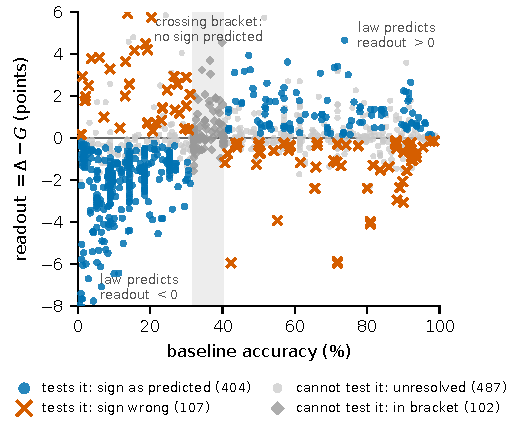
\includegraphics[width=\linewidth]{figs/law_scatter.pdf}
\caption{The law, in full: \readout{} $=\Delta-G$ against baseline accuracy
for all \auditScope{} law-scope cells with ${\geq}3$ seeds on both arms. Shaded
band: the measured crossing bracket $[31.8,40.3]$, inside which no sign
is predicted. Only the first two legend entries test the account: of the \auditResolvable{}
cells whose \readout{} is resolvable against its own seed-paired uncertainty,
\auditCorrect{} fall on the predicted side of zero. The other two entries keep the audit's reach visible:
\auditUnresolved{} are unresolvable and \auditBracket{} sit inside the
bracket, so the rate is $\auditRate\%$ at $\auditCoverage\%$ coverage against a
$\auditMajority\%$ majority-sign baseline.
The scatter at fixed baseline is substantial ($R^2 = 0.27$, residual SD
$\auditResidSD$ points): the account predicts the sign of this term, not its value.}
\label{fig:law}
\end{figure}

\looseness=-1 That regularity is not a theorem but an empirical one with measured scope,
registered in advance (Sec.~\ref{sec:lawpredict}) and found only after two
wrong intermediate laws, a ``deficit'' law and a multiplicative
realization$\times$gain form, were falsified by our own cells and retracted.
Its content is asymmetric: below the crossing it predicts a large negative
\readout{} and is strongly falsifiable; far above it predicts \readout{}
${\approx}0$, true but weakly discriminating, so a naive sign-count over
high-data cells would produce a coin flip and wrongly suggest failure. The
audit therefore counts only cells whose \readout{} is resolvable against its own
\emph{seed-paired} uncertainty (Sec.~\ref{sec:stats}), tighter than
independent propagation and the protocol the released script implements.

\subsection{The audit}\label{sec:lawaudit}
\begin{table}[pos=htbp]
\caption{Scope-wide sign-law audit, regenerated from the per-run records by the
released audit script. A cell is resolvable when $|\readout| > 2\,\mathrm{SEM}$; cells inside
the crossing bracket make no sign prediction. Uncertainty is seed-paired
(Sec.~\ref{sec:stats}), not propagated from independent arms. Scope is
aux-from-scratch: cells carrying an ImageNet or self-supervised
initialization are excluded here and scored separately in
Sec.~\ref{sec:fusion}, and $100\%$ cells report only the aux-vs-baseline
gap under the scope rule of Sec.~\ref{sec:probe}, which is why the
first row is much larger than the
second; the rows narrow to the resolvable subset that actually tests the
account.}
\label{tab:audit}
\centering\scriptsize
\setlength{\tabcolsep}{2.6pt}
\zebra{2}
\begin{tabular}{lr}
\toprule
Population & Cells \\
\midrule
Cells with paired $\Delta$ and $G$ (all interventions) & \auditAllPaired \\
\quad in scope, ${\geq}3$ seed-matched arms & \auditScope \\
Backbone variants in scope (architecture families) & 7 (5) \\
Dataset identities in scope & 20 \\
Inside crossing bracket (no prediction) & \auditBracket \\
Unresolved ($|\readout| \le 2$\,SEM) & \auditUnresolved \\
\midrule
\textbf{Resolvable (these test the account)} & \textbf{\auditResolvable} \\
\quad Sign as predicted & \textbf{\auditCorrect{} (\auditRate\%)} \\
\quad Wrong side & \auditWrong \\
\bottomrule
\end{tabular}
\end{table}

\begin{table}[pos=htbp]
\caption{Robustness of the audit: the rate is stable against the
resolvability threshold, survives clustering on the units that share a
baseline arm, and survives re-fitting the crossing bracket without the
audited dataset (the out-of-sample check). It is carried by
the left flank, where the account predicts strongly, not by the
right, where it predicts ${\approx}0$. Intervals are Wilson 95\%.}
\label{tab:robust}
\centering\scriptsize
\setlength{\tabcolsep}{2.6pt}
\zebra{2}
\begin{tabular}{P{0.30\columnwidth}rrrP{0.20\columnwidth}}
\toprule
Audit variant & Cells & Correct & Rate & 95\% CI \\
\midrule
$|\readout| > 1$\,SEM & 629 & 509 & 80.9\% & [77.7, 83.8] \\
$>1.5$\,SEM & 531 & 446 & 84.0\% & [80.6, 86.9] \\
\textbf{$>2$\,SEM (declared)} & \textbf{\auditResolvable} & \textbf{\auditCorrect} & \textbf{\auditRate\%} & \textbf{[82.9, 89.2]} \\
$>3$\,SEM & 342 & 304 & 88.9\% & [85.1, 91.8] \\
\midrule
One vote per (dataset, backbone, fraction) & 235 & 192 & 81.7\% & [76.3, 86.1] \\
Held out: bracket fitted without the audited dataset & 391 & 347 & 88.7\% & [85.2, 91.5] \\
\midrule
Below the crossing & 314 & 298 & 94.9\% & [91.9, 96.8] \\
Above the crossing & 141 & 95 & 67.4\% & [59.3, 74.6] \\
\bottomrule
\end{tabular}
\end{table}

\looseness=-1 Table~\ref{tab:audit} summarizes the audit: of \auditResolvable{} resolvable
cells spanning seven backbones and nineteen of the twenty dataset identities
in scope (the caption of Table~\ref{tab:partitions} explains why identities
outnumber image sources; one has law-scope cells but no resolvable one), \auditCorrect{}
($\auditRate\%$) fall on the predicted side (Wilson 95\% CI $[82.9, 89.2]$).
Eleven cells entered scope late, ten of them resolvable, when the
prior-with-augmentation arms of Sec.~\ref{sec:stack} and the fixed-step
cells acquired their frozen-feature evaluations. All
are aux-from-scratch cells with both measurements, so the law's own definition
admits them, excluding them after seeing their effect would be the
selection this benchmark exists to expose, and admitting them lowered the
rate by three-tenths of a point, on overlapping intervals.

\looseness=-1 Two numbers belong beside that one. The resolvability rule decides which
cells vote, and only $\auditCoverage\%$ of scope cells do, so we write the
result as $\auditRate\%$ \emph{at $\auditCoverage\%$ coverage} throughout.
The null matters as much: an exact binomial against a coin returns $p \approx
2\times10^{-58}$, true and useless, because nobody proposes a coin. The
\readout{} term is
negative in most resolvable cells, so always predicting negative already
scores $\auditMajority\%$; the account beats that, but the honest effect size
is the gap to $\auditMajority\%$, not to $50\%$. Below the crossing, where
the account makes a strong prediction, it is $298/314 = 94.9\%$; above it,
where it predicts only that the term is small, $95/141 = 67.4\%$. The
\auditWrong{} exceptions group rather than scatter. One carries a single
signature, $G$ clearly positive while $\Delta$ is negative at ${\geq}20\%$ data
on Food-101 and PathMNIST, ``better features, worse accuracy at sufficiency''.
A second is an artifact of the account's \emph{input}, not its prediction: the
two largest exceptions are Swin cells whose baseline arm is seed-bistable, so
their nominal baseline height averages trained and collapsed seeds and does not
measure how well the task is being solved. We leave them in the count and name
them instead: dropping bistable-baseline cells would raise the reported rate,
so excluding them is not a neutral choice. Table~\ref{tab:exceptions} lists the largest-magnitude exceptions
individually, because where an account fails is part of what it claims.

\paragraph{Two scope repairs that moved this number, and by how much.}
\looseness=-1 An earlier version of this audit reported $\auditPrevRate\%$
over $\auditPrevResolvable$ resolvable cells from a scope of
$\auditPrevScope$; the figure is higher because two scope filters were
repaired, not because any run, seed or measurement changed. First, cells
carrying an ImageNet initialization, the interference case of
Sec.~\ref{sec:taxsub} and outside the regime the \readout{} branch was
estimated in, leaked in through a string mismatch: the filter tested the
exported \texttt{pretrained} field against \texttt{true} and \texttt{1}
while the exporter writes \texttt{yes}. Restoring it removes
\auditExclCells{} cells, \auditExclResolvable{} of them resolvable
(\auditExclCorrect{} correct, \auditExclWrong{} wrong,
$\auditExclRate\%$ on their own), taking the scope to $\auditMidScope$
and the rate to $\auditMidRate\%$ over \auditMidResolvable{} resolvable
cells; below the
crossing the $298$ correct cells are untouched while $23$ wrong ones leave
($\auditPrevBelowRate\%$ to $\auditMidBelowRate\%$),
Sec.~\ref{sec:taxsub} seen from the other side. Second, at $100\%$ cells
Sec.~\ref{sec:probe} reports the aux-vs-baseline gap and refuses the
$G$/\readout{} split, yet the released script carried no such filter.
Removing the \auditHundredCells{} full-data cells drops
\auditHundredResolvable{} resolvable cells (\auditHundredCorrect{} correct,
\auditHundredWrong{} wrong, $\auditHundredRate\%$ on their own, the
worst-scoring subset in the audit and exactly the cells the rule calls
uninterpretable), moving the headline from $\auditMidRate\%$ to
$\auditRate\%$ and the below-crossing flank to $\auditBelowRate\%$
(\auditHundredBelow{} more cells, both wrong). The price is breadth: ViT-S,
ViT-B and ImageNet-100 hold law-scope cells only at $100\%$, so the span
narrows from nine backbones to seven and from twenty-one dataset identities
to twenty, though the five architecture families survive. Both pre-repair
headlines and both excluded subsets' own rates are stated above so the
repair stays visible. Sec.~\ref{sec:scale} is untouched:
Table~\ref{tab:scale} reports $\Delta$, $G$ and their gap with no signed
\readout{}, which the rule permits, so the ImageNet $\Delta \approx G$
result stands while the same cells leave the sign-law count.

\begin{table}[pos=htbp]
\caption{The ten largest-magnitude resolvable exceptions, of
\auditWrong{} in total, printed from the same audit as
Table~\ref{tab:audit}; they cluster, not scatter. \emph{Top:} Swin cells
whose baseline arm is unstable (seed SD $10$--$22$ points), so the baseline
height the account takes as input is not a task-performance reading; the
records flag the first two as bistable and the third narrowly not.
\emph{Second:} the ``better features, worse accuracy at sufficiency''
signature. \emph{Third:} PathMNIST, whose linear evaluation is a compressed
measuring stick. \emph{Bottom:} two heavily-augmented ViT cells on DTD, with
\readout{} positive far below the crossing.}
\label{tab:exceptions}
\centering\scriptsize
% 8 columns = 16 gutters, so each 0.1pt here is 1.6pt of width. At 2.6pt this
% ran 3.01pt over the measure. Narrowing the gutter also shrinks the zebra
% overhang, which is \tabcolsep on each side, so it stays inside the rules.
\setlength{\tabcolsep}{2.3pt}
\zebra{2}
\begin{tabular}{lllrrrrr}
\toprule
Dataset & Backbone & Variant & Frac. & Base & $\Delta$ & $G$ & \textit{Readout} \\
\midrule
EuroSAT & Swin & aux & 20\% & 22.7 & $+71.27$ & $+55.93$ & $+15.34$ \\
EuroSAT & Swin & aux & 15\% & 18.6 & $+73.72$ & $+61.66$ & $+12.06$ \\
EuroSAT & Swin & aux & 2\%  & 42.3 & $+30.54$ & $+36.49$ & $-5.95$ \\
\midrule
Food-101 & R18 & mag3 & 50\% & 71.8 & $-1.30$ & $+4.66$ & $-5.96$ \\
Food-101 & R18 & mag6o & 50\% & 71.8 & $-0.91$ & $+4.97$ & $-5.88$ \\
Food-101 & MNet & aux & 50\% & 55.1 & $-0.23$ & $+3.70$ & $-3.93$ \\
\midrule
PathMNIST & R18 & mag6o & 1\% & 80.8 & $+5.80$ & $+9.90$ & $-4.09$ \\
PathMNIST & R18 & mag3 & 1\% & 80.8 & $+5.62$ & $+9.60$ & $-3.98$ \\
\midrule
DTD & ViT & deit-aux & 100\% & 13.2 & $+25.55$ & $+21.91$ & $+3.63$ \\
DTD & ViT & deit-aux & 50\% & 14.2 & $+17.30$ & $+14.73$ & $+2.57$ \\
\bottomrule
\end{tabular}
\end{table}

Table~\ref{tab:robust} reports what that number survives. Not the resolvability
threshold: the rate moves only from $80.9\%$ over 629 cells at one SEM to
$88.9\%$ over 342 at three, so a stricter or looser criterion reaches the same
conclusion. Not the dependence between cells: collapsing to one vote per
(dataset, backbone, fraction) leaves $192/235 = 81.7\%$. And, the check that
matters most, not the estimation of the crossing bracket on the cells we then
audit: re-fitting it on the other datasets and auditing each dataset out of
sample gives $347/391 = 88.7\%$, indistinguishable from the in-sample figure.

That row audits 391 cells, not all \auditResolvable{}, and the shortfall is not
a sampling choice. Re-fitting the bracket on the other datasets widens it
beyond the pooled $[31.8, 40.3]$, since one dataset's cells no longer pin
either edge (for CIFAR-100 it becomes $[29.5, 71.0]$), and cells inside a
bracket make no sign prediction, so $46$ leave the held-out set that way, 25 of
them CIFAR-100's; a further $18$ sit in datasets that cannot receive a fold
($391 + 46 + 18 = \auditResolvable$). The bias runs one way: the held-out row
keeps the cells furthest from the crossing, where the account is most
confident, so its rate is a mild upper bound rather than a like-for-like
comparison, and the effect is small since $86\%$ of resolvable cells do receive
an out-of-sample verdict.

What the number does \emph{not} survive is disaggregation. The evidence is
overwhelmingly left-flank: below the crossing the sign is right $94.9\%$ of the
time, above it $67.4\%$, close to a coin once the term it predicts has shrunk
to nothing. One dataset behaves badly out of sample, PathMNIST at $52.6\%$: its
linear evaluation is a known compressed measuring stick, its frozen-feature
accuracy sitting \emph{below} its own end-to-end accuracy, so we treat its
$G$ as unreliable there, not the account as refuted, and report the failure
instead of excluding the dataset. We do not explain this cluster; we name it
as the law's known boundary (Sec.~\ref{sec:limits}), and the released audit
script enumerates every exception.

\paragraph{What the \readout{} term is, once the label budget is matched.} Every
$G$ above uses one evaluation budget for all cells, the full training split,
while the cell itself trained on a fraction of it: at $1\%$ the evaluation
holds a hundred times the cell's labels. That asymmetry could on its own
explain the negative branch, so we measured it, re-evaluating both arms of $30$
reference-configuration cells across seven datasets, baselines $5.3$ to $93.8$, at \emph{each
cell's own} per-class budget (five to $2{,}500$ labels per class).

The stronger result comes first. At matched budget the end-to-end gain and the
frozen-feature gain agree to $0.17$ points on average, median $0.11$ and worst
case $0.77$, against $0.89$ under the full-label protocol. A linear evaluation
run at the label budget a practitioner actually has therefore predicts the
end-to-end difference between two arms without training either combination, and
what had been a two-cell observation now holds over $30$ cells and seven
datasets.

The second result follows from it and cuts against our own framing, which is
why we registered it in advance. The \readout{} term largely disappears at matched
budget: below the crossing its mean moves from $-1.66$ to $-0.19$ and above it
from $+0.10$ to $-0.13$, $19$ of $30$ cells lose more than half their
magnitude, and only $3$ of $30$ stay resolvable against their own uncertainty.
Below the crossing the negative sign is thus substantially a statement about
the ratio of evaluation labels to training labels, for which baseline accuracy
is a monotone proxy, rather than an independent property of training. The sign
law remains an accurate description of the full-label protocol, the protocol
every $G$ in this paper is measured under, so Tables~\ref{tab:audit} and
\ref{tab:robust} stand exactly as measured; what changes is how to read them.

\subsection{Prediction, not description}\label{sec:lawpredict}
Three pre-registered episodes distinguish the law from a post-hoc fit.

\emph{(i) A new backbone family from baselines alone.} Before any Swin-T linear
evaluation existed, we read the \readout{} term off the measured curve at Swin's
baseline heights and published bands for its feature gain ($G \approx 9.6$,
$8.8$, $9.8$ and $7.0$ at 5, 10, 15 and 25\% of CIFAR-100; band $+7$--$+11$).
The measurements landed at $10.5$, $9.3$, $10.1$, $7.6$: four of four in band,
each within one point of its point call, against two live falsifiers
(attention-intrinsic $G{\geq}13$; stabilization-only $G{\leq}6$), either of
which would have refuted the account.

\emph{(ii) Four unseen domains.} The same procedure applied to satellite,
texture, food and histopathology cells straddling the crossing produced eight
banded predictions; seven landed in band and all eight had the predicted sign,
including the two deliberately hard cases where a small $\Delta$ could have
hidden a large $G$ (it did not: small $\Delta$ meant small $G$).

\emph{(iii) ImageNet scale}, the subject of Sec.~\ref{sec:scale}, where the
residual $\Delta - G$ was pre-registered to stay within $1.5$ points on every
backbone.

\subsection{What $G$ is a function of}\label{sec:lawG}
Controlled crossings localize the law's terms. $G$ is a property of the
checkpoint and the evaluation's label space. It is invariant to which coarse
partition relabels the data, but is cut roughly from $4.2$ to $2.9$ when
training supervision moves from 200-way fine to 20-way coarse labels on
identical pixels: fine-grained weak supervision is where the prior has the most
feature work to do. The \readout{} term follows task performance, not label
budget: engineered cells that lower class count without raising baseline
accuracy get no \readout{} boost (a prediction our own account initially got
wrong, and the cell that corrected it is in \ref{app:controls}). And
$G$ depends on the backbone as sharply as on the data: at the same
Tiny-ImageNet cell, ResNet-18 carries $G = +2.66$ while MobileNetV3 carries $G
= +0.01 \pm 0.23$, a measured zero on the weaker network, so ``how much a prior
can add'' is not a dataset property but a (dataset, architecture) property.

\subsection{What the prior leaves behind}\label{sec:imprint}
\begin{figure}[pos=htbp]
\centering
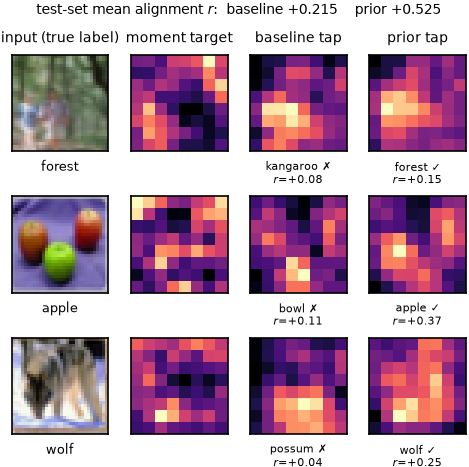
\includegraphics[width=\linewidth]{figs_explain/heatmaps_auxmag_5pct_sched0.png}
\caption{The spectral imprint at the tap, CIFAR-100 at 5\%. Columns:
input, the fixed moment target, and the tapped-stage energy of the
baseline and prior arms. Over the \emph{whole} test set the alignment
between tapped features and the target is $+0.215$ for the baseline and
$+0.525$ for the prior arm. The three rows are \emph{selected} cases
(prior arm correct, baseline wrong), so they illustrate the alignment
difference, not sample it, and only the test-set-wide figure
should be read as evidence.}
\label{fig:heatmap}
\end{figure}
$G$ is a number, and it is worth seeing what in the representation it
corresponds to. The prior's target is a fixed bank (Fig.~\ref{fig:bank}), and
its imprint survives to the end of training: at the CIFAR-100 5\% cell, where
the feature gap is largest on this dataset ($+6.3$ points), the alignment
between tapped features and the bank's oriented-energy target measured over the
whole test set is $+0.525$ for the prior arm against $+0.215$ for the baseline
(Fig.~\ref{fig:heatmap}). That it survives is the part that matters, because the auxiliary weight
decays to exactly zero well before training ends: the prior changes where the
representation settles, not what the loss pulls on at the finish.

\begin{figure}[pos=htbp]
\centering

\includegraphics[width=\linewidth]{figs_explain/cam_auxmag_5pct_sched0.png}
\caption{Where the class evidence sits, CIFAR-100 at $5\%$. The three rows are
\emph{selected} cases (prior arm correct, baseline wrong), so they show what the
difference looks like where it is present, not how often. The evidential
quantity is measured over the whole test set instead: the Gini coefficient of
each class-activation map normalized to sum one, where higher means evidence
concentrated at fewer locations, gives $\camBase$ for the baseline against
$\camAux$ for the prior arm over $\camN$ images ($\camSigma\,\sigma$). The
prior's evidence is measurably more
concentrated, by a modest amount, not the categorical difference the three
rows suggest.}
\label{fig:cam}
\end{figure}

A second, independent read asks not what the features encode but where the
class evidence sits: Fig.~\ref{fig:cam} scores the concentration of each
class-activation map over the whole test set, and the prior's evidence is
measurably more concentrated, though only by $+\camDelta$.

\paragraph{Is that imprint specific, or is it what good features look like?}
One cell cannot tell the two apart, and any intervention that improves features
might show the same alignment, so we measured the same statistic across
families that reach a positive $G$ by \emph{different} routes, against one
pinned target for every model, since a self-supervised initialization has no
auxiliary head and therefore no target of its own. Reporting the alignment gap,
each arm minus its own baseline (Table~\ref{tab:imprint},
Fig.~\ref{fig:imprint2}):

\begin{table}[pos=htbp]
\caption{The imprint follows the \emph{target}, not the feature gain.
Alignment gap is the arm minus its own baseline, CIFAR-100/ResNet-18, one
pinned target applied to every model. The lower block is a $2\times2$ that
fell out of the design: crossing \{self-supervised initialization or not\}
with \{moment target or not\}, the imprint tracks the target while $G$
tracks the initialization. Best in bold, second best underlined, third best
in italics, per numeric column; the two columns' markings disagree.}
\label{tab:imprint}
\centering\scriptsize
\setlength{\tabcolsep}{4pt}
\zebra{2}
\begin{tabular}{lrrr}
\toprule
Family & $n$ & mean $G$ & alignment gap \\
\midrule
Moment prior (tap L3)        & \imprintPriorN & $+\imprintPriorG$ & \snd{$+\imprintPrior$} \\
SimCLR init, no target       & \imprintSSLN   & \snd{$+\imprintSSLG$}   & $\imprintSSL$ \\
Random fixed target          & 1              & $+1.31$           & \trd{\imprintRand} \\
\midrule
Moment prior, tapped at L1/L2 & 2 & \trd{+4.67} & $\imprintTap$ \\
SimCLR init $+$ moment target & 1 & $\mathbf{+8.08}$ & $\mathbf{+\imprintCombo}$ \\
\bottomrule
\end{tabular}
\end{table}

\begin{figure}[pos=htbp]
\centering
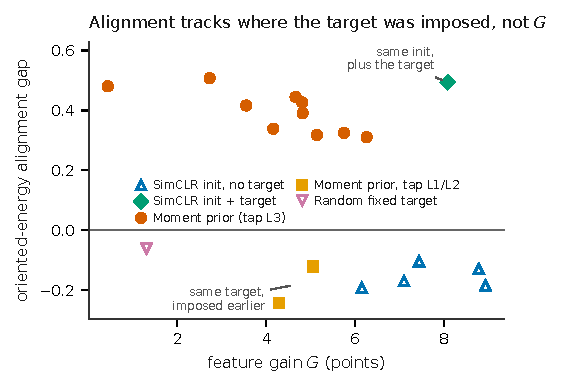
\includegraphics[width=\linewidth]{figs/imprint_dissociation.pdf}
\caption{Alignment gap against feature gain, one point per cell, CIFAR-100 /
ResNet-18. Filled markers had the moment target during training. The two
quantities are independent: every cell whose target was imposed at the tapped
stage sits at $+0.31$ to $+0.51$ regardless of whether its $G$ is $2.7$ or
$8.1$, and every cell without a target there sits below zero across the same
range of $G$. The two labelled controls separate the accounts: the
same target imposed two stages earlier leaves no imprint at layer~3, and the
same self-supervised initialization as the negative points, with the target
added, gives the largest gap measured.}
\label{fig:imprint2}
\end{figure}

The self-supervised cells are the decisive comparison and they answer it in the
strongest available direction: they carry \emph{more} feature gain than the
prior ($G = +\imprintSSLG$ against $+\imprintPriorG$) and \emph{less}
oriented-energy structure than their own baselines ($\imprintSSL$). We had
registered a band of $-0.05$ to $+0.10$ for them and a falsifier at $\geq
+0.15$; the measurement came back at the opposite sign, so oriented-energy
alignment is not simply what better features look like on this data.

Two controls fell out of the design unplanned, and each isolates one factor
more sharply than the comparison we set out to make. Moment-prior cells
\emph{tapped two stages earlier} use the identical target and show
$\imprintTap$ when read at layer~3: the imprint is localised to where the
target is imposed, which a mechanism predicts and an incidental correlation
does not. And a cell with the same SimCLR initialization as the $\imprintSSL$
rows, plus the moment target, shows $+\imprintCombo$, the largest gap we
measure. Crossed, these give a $2\times2$ in which the imprint follows the
target and $G$ follows the initialization.

What this does \emph{not} establish: alignment is a correlation between
channel-\emph{mean} energy maps, so it measures agreement in spatial layout,
not reproduction of the individual oriented channels, and a null on it would
not rule out a finer imprint. The two control rows are single cells.

\begin{figure}[pos=htbp]
\centering
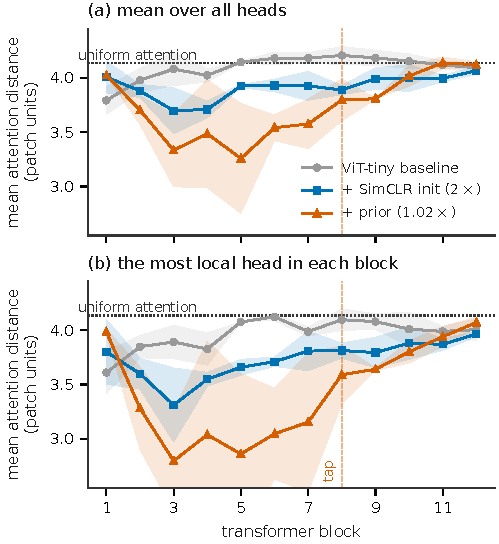
\includegraphics[width=\linewidth]{figs/attention_locality.pdf}
\caption{What the prior gives a small transformer: locality. Mean
attention distance per block, ViT-tiny on CIFAR-100 at 10\%, three seeds
(band: $\pm$1 SD). The dotted line is the distance a \emph{uniform} attention
map would give on this $8\times8$ token grid ($4.14$ patch units), computed, not assumed. The baseline sits on that line at every depth, never
learning to attend locally from 5{,}000 images; the prior
pulls the middle blocks well below it, most sharply \emph{upstream} of the
tap. A SimCLR initialization at $2\times$
the compute does the same, more weakly.}
\label{fig:attention}
\end{figure}
The same question can be put to the backbone where the prior matters most,
and there the answer is unusually legible. A vision transformer has no
built-in notion that nearby patches belong together; the standard diagnostic
for whether it has learned one is mean attention distance.
Figure~\ref{fig:attention} measures it for ViT-tiny at CIFAR-100 10\%: the
baseline's heads straddle the uniform-attention distance at every depth, never
discovering locality on 5{,}000 images, while the prior pulls the middle
blocks well below it. The prior does not merely improve the features; it
supplies the spatial inductive bias the architecture lacks, which a
convolutional backbone gets for free and is why the same intervention is worth
several times more here.

We had predicted this effect in the \emph{early} blocks, decaying with depth,
and that is not what happened: at block~1 the ordering is nominally reversed,
the effect peaks at blocks~3--7, and the curves rejoin by block~11. The
location is interpretable after the fact, since the target is regressed from
block~8 and the locality appears in the blocks that feed it, but we did not
predict it and record it as a missed call on a held prediction, not a
confirmation. A SimCLR initialization produces the same signature at about half
the depth-integrated magnitude, which is consistent with the two being
substitutes on this backbone.

We are deliberate about how far the qualitative evidence goes. The
individual-image maps of Figs.~\ref{fig:heatmap} and \ref{fig:cam} are
selected on cases the prior gets right
and the baseline wrong, so they illustrate rather than demonstrate; a t-SNE
of the frozen features (Fig.~\ref{fig:tsne}) moves the all-class silhouette
only from $-0.072$ to $-0.064$, since a $+6.3$-point feature gap need not be
legible in two projected dimensions. The alignment statistic and the linear
evaluation are the measurements; the pictures illustrate them.

%% ---------------------------------------------------------------------
\section{Fusion outcomes: stack, substitute, interfere}\label{sec:fusion}

The grid's central comparative finding is that fusion outcomes are predictable
from the \emph{currency} each information source supplies.

\textbf{What we mean by currency, operationally.} The word is a metaphor
used once as one; what it stands for is a measurement from single-source
quantities only, so nothing in it requires training the combination. A
source's currency is characterised from that source \emph{alone}: the
frozen-feature gain $G$ it produces under the declared protocol, together
with \emph{what} it improves, that is, which test images its arm fixes and
how similar its learned representation is to the other source's, both
measured on the single-source arms (Sec.~\ref{sec:samecurrency}). Two
sources trade in the same currency when, at a matched cell, their $G$ values
agree \emph{and} their single-source arms agree, on images fixed and in
representation, about as closely as two seeds of one source do; both halves
are necessary because two representations can raise linear accuracy equally
while encoding different things. The combination's $G$ appears nowhere in
the definition; it is what the definition \emph{predicts}, same currency
implying that the combination's $G$ will not exceed the better single
source, and Secs.~\ref{sec:substitute} and~\ref{sec:samecurrency} test
that prediction. $G$ is a cheap ordinal proxy for source overlap, not an
estimate of the unique and redundant atoms that partial information
decomposition formalizes (Sec.~\ref{sec:fusiontheory}); what it buys is
measurability on each source alone, at the cost of one linear fit, which is
what makes a prospective rule possible at this grid's scale.

This section presents the three outcomes in order of how favorable they are:
different currencies can compound, differing currency being necessary while
architecture and intervention strength decide how much is realized
(Sec.~\ref{sec:stack}); the
same currency
adds nothing, with the refinement that rescues the rule from its apparent
counterexamples (Sec.~\ref{sec:substitute}); and one fusion, at full
shaping strength, is uniformly
destructive, with the feature-level measurement that explains why
(Sec.~\ref{sec:taxsub}). Section~\ref{sec:taxonomy} collects the three
into a single table with the evidence for each row.

\subsection{Different currencies can stack}\label{sec:stack}
DeiT-strength augmentation supplies invariance to nuisance transforms; the
prior supplies oriented-energy structure. Fusing both
(Table~\ref{tab:vitenvelope}) does not trade off: the prior's ViT gain grows
under augmentation on both populations, by $1.5$--$2.4\times$ on CIFAR-100 and
$1.4$--$2.4\times$ on Tiny-ImageNet across $1$--$25\%$. We give the two ranges
separately because we once gave one: a registered ``$1.8$--$2.4\times$
throughout'' missed low on Tiny-ImageNet at 5, 15 and $25\%$, so amplification
is population-dependent and the CIFAR-100 range was over-generalized. On
Tiny-ImageNet it also vanishes at full data ($0.92\times$), where both
interventions are decaying anyway. The feature side confirms the mechanism: the prior's $G$
\emph{rises} under augmentation (from $14.8$ to $22.2$ at 10\%), because once
nuisance variation is handled the network can commit more capacity to the
structure the target teaches. Our own pre-registered bet here was wrong in the
pessimistic direction: we predicted partial substitution and measured strong
complementarity.

\paragraph{How far that reaches, on a convolutional backbone.} Every cell
above is a ViT, on CIFAR-100 (the selection set) or Tiny-ImageNet (no part in
selection, Sec.~\ref{sec:selection}). What the result does not span is a
convolutional backbone off the selection set, so we ran the three missing
fusion arms there, augmentation alone, prior with augmentation, and prior
with a SimCLR initialization, on EuroSAT and Food-101 with ResNet-18 at 5, 10
and $25\%$. The substitution result transplants; the stacking result does
not.

\looseness=-1 Prior with SimCLR falls below the better single source at all six cells
($-0.14$ to $-2.41$), so on these convolutional populations it does not merely
fail to add, it costs, and the registered falsifier for the substitution rule,
a combination beating the better single by ${\geq}1.5$, fired nowhere. Prior
with augmentation stacks at exactly one cell of six, Food-101 at $5\%$
($+4.32$, eleven standard errors), and is negative at the other five ($-0.37$
to $-3.07$). That tripwire required failure on \emph{both} populations, so it
did not fire on the letter; we report it as a narrowing rather than a pass.
Prior-with-augmentation stacking is therefore a result about attention
backbones, holding on both the selection population and an off-selection one,
plus a single convolutional cell; it is not a general property of the two
currencies.

\looseness=-1 What does hold across these cells and the schedule control of
Sec.~\ref{sec:taxsub} concerns strength. Adding the prior at full weight
costs whenever the partner is already strong: where augmentation is harmful the
prior leads (EuroSAT at $5\%$, augmentation alone $-7.67$ against the prior's
$+0.84$), and where augmentation is strong the prior subtracts (Food-101 at
$10\%$, augmentation alone $+9.26$, adding the prior $-1.81$). Frozen-feature
evaluation of the same arms agrees: measured against the same partner alone,
the prior moves $G$ by $+4.68$, $-1.22$ and $-1.51$ on Food-101 over
augmentation at 5, 10 and $25\%$, and by $-1.38$, $-2.29$ and $-1.27$ over the
SimCLR initialization, so the cost is feature-side here as for the transfer
tax. One more thing the attention-only evidence had hidden: DeiT-strength
augmentation is not universally good, worth $+9.45$, $+9.26$ and $+3.05$ alone
on Food-101 but $-7.67$, $-0.14$ and $+0.11$ on EuroSAT, so a claim about
augmentation as a fusion source has to name its domain.

\subsection{Same currency substitutes}\label{sec:substitute}
\begin{table}[pos=htbp]
\caption{Prior versus SimCLR initialization ($2\times$ compute) on
ViT-tiny, CIFAR-100, and the effect of recipe. Under plain augmentation
SSL catches the prior at ${\sim}5$k images; under the DeiT recipe the
prior wins at every fraction because the recipe supplies the invariance
SSL was selling. Three seeds per cell, six on the DeiT-recipe $5\%$ arm. A positive entry is a fraction
where the prior wins; no better-direction marker is used, since neither
sign of a method-versus-method difference is better a priori. Per fraction
the recipe under which the prior stands better is bold; with two rows the
second-best and third-best marks do not apply.}
\label{tab:flip}
\centering\scriptsize
\setlength{\tabcolsep}{2.6pt}
\zebra{4}
\begin{tabular}{lrrrrr}
\toprule
 & \multicolumn{5}{c}{prior $-$ SimCLR (points)} \\
\cmidrule(l){2-6}
Recipe & 1\% & 5\% & 10\% & 25\% & 100\% \\
\midrule
Plain crop+flip & $+0.7$ & $+1.3$ & $0.0$ & $-1.4$ & $-3.9$ \\
DeiT augmentation & $\mathbf{+2.5}$ & $\mathbf{+7.2}$ & $\mathbf{+5.2}$ & $\mathbf{+5.0}$ & $\mathbf{+2.0}$ \\
\bottomrule
\end{tabular}
\end{table}

\looseness=-1 SimCLR's objective \emph{is} invariance to an augmentation family. Three
measurements pin the consequence. First, prior and SimCLR never stack: on
convolutional backbones the combination costs $-1.5$ points against SimCLR
alone, and on ViT it is exactly neutral against the better single arm. Their
feature gains are the same gain ($G = 14.8$ against $13.5$ at the same cell),
so the second source has nothing left to add. Second, the head-to-head flips
with the recipe (Table~\ref{tab:flip}): under plain augmentation SSL overtakes
the prior once data is plentiful, but under the DeiT recipe, the recipe anyone
training a small ViT would actually use, the prior wins at every CIFAR-100
fraction, by ${\sim}5$ points across the mid-band, and the feature side shows
why: augmentation lifts the prior's $G$ by $+7.4$ but SimCLR's by only $+3.8$
at 10\%. The same flip reproduces on Tiny-ImageNet in the low-data band. Third,
SimCLR was not under-equipped: giving its contrastive views DeiT strength makes
it \emph{worse} at every fraction (by $4$--$12$ points e2e, halving its $G$),
so its standard configuration was its strongest available one.

The substitution rule refines rather than universalizes: fusing the prior onto
\emph{ineffective} SSL stacks trivially. SimSiam at its published
budget learns almost nothing at study scale ($\Delta \leq +0.9$ at every
CIFAR-100 and CIFAR-10 fraction, ${\leq}+1.8$ on any population), and
prior-on-SimSiam recovers the prior's full gain ($+6.2$ and $+4.3$ over
SimSiam alone at CIFAR-100 5 and 10\%, and $+2.0$ at Tiny-ImageNet 5\%). The operative rule is therefore \emph{the prior is
redundant exactly insofar as the other source already bought the same
features}, judged by the other source's own measured gain, not by its family
name.

\looseness=-1 The grid contains the intermediate case, and it contradicts the binary phrasing
of Table~\ref{tab:taxonomy}'s second row while supporting the rule just stated.
On ViT-tiny at CIFAR-100, prior with a DINO initialization beats the better
single arm by $+0.92$ at $10\%$ ($30.66$ against the prior's $29.74$, about
five standard errors) and $+1.02$ at $5\%$ ($22.62$ against $21.60$), and a
combination exceeding both singles is what that row says cannot happen. The
refined rule predicts it: DINO is a partial source here, its feature gain
$+7.90$ roughly half the prior's $+14.83$, so it has not bought the same
features and work is left for the prior to do. The feature side confirms rather
than merely permits that reading, since the combination's $G$ is $+14.77$,
level with the prior alone, not above it: the two still substitute in
feature space even as the combination edges ahead end to end. We therefore state the row as \emph{combination $\leq$ best
single when the partner's $G$ matches the prior's, and partial when it does
not}, and we count these cells as the case that forced the qualification.

\subsection{Fusing into mature features interferes}\label{sec:taxsub}
\begin{table}[pos=htbp]
\caption{The interference tax of the ImageNet-transfer fusion, and its
feature-side origin. Injecting the
prior on top of ImageNet weights \emph{at full auxiliary strength} is
destructive in proportion to what the initialization supplied; linear
evaluation shows the loss is carried almost entirely by $G$ (features), not by
the \readout. PathMNIST, where ImageNet features barely transfer, is the null
control. Ten seeds on the two CIFAR pairs end-to-end, three on PathMNIST, and
three for every linear evaluation, so the \readout{} column differences a
ten-seed $\Delta$ against a three-seed $G$. The text below reports the same
three cells at reduced $\lambda_0$, where the tax disappears.}
\label{tab:tax}
\centering\scriptsize
\setlength{\tabcolsep}{2.6pt}
\zebra{2}
\begin{tabular}{lrrrrr}
\toprule
Dataset & Frac. & Transfer adv. & $\Delta$ (tax)~\up & $G$~\up & \textit{Readout} \\
\midrule
CIFAR-10 & 5\% & $+9..{+}14$ & $-15.2$ & $-15.8 \pm 1.7$ & $+0.6$ \\
CIFAR-100 & 7\% & $+10..{+}18$ & $-16.8$ & $-16.3 \pm 3.1$ & $-0.6$ \\
PathMNIST & 10\% & $+1.8..{+}2.9$ & $-0.4$ & $+0.3 \pm 0.6$ & $-0.7$ \\
\bottomrule
\end{tabular}
\end{table}

The one uniformly destructive fusion in the grid is instructive
(Table~\ref{tab:tax}). The prior's early shaping at full strength, so valuable
from scratch, \emph{erases} mature ImageNet features. We call the measured
degradation an \emph{interference tax}, and the tax runs $-15.2$ to
$-16.8$ on the two datasets where
transfer was worth $+10$ to $+18$ on the cells of Table~\ref{tab:tax}, decays
to zero at full data (where the initialization no longer carries the
performance), and, the decisive measurement, lands almost entirely on $G$.
Where the initialization had little to offer (histopathology), there is nothing
to destroy and the tax is a measured zero. Fusion with an information-rich
partner must respect what the partner already encodes; a shaping prior does
not.

Table~\ref{tab:tax} shows the three cells we could also probe, and three cells
cannot carry a claim about a regime, so we state the population they come from:
of the \taxCells{} transfer cells that carry the prior \emph{at full auxiliary
strength from the first step} ($\lambda_0 = 1.0$, no delayed onset) at three or
more seeds, \taxNegative{} have a
negative $\Delta$, spanning nine datasets, with a median of $\taxMedian$ and a
worst case of $\taxWorst$. Not one is positive.

Full strength defines that population rather than describing it, so the
released records hold more aux-on-pretrained cells than the figure counts: the
reduced-strength and delayed arms below are the \emph{control} for this claim,
and counting them inside the population they exist to explain would remove the
``not one is positive'' by construction while establishing nothing. What the
\taxCells{} cells establish is that \emph{this} shaping schedule interferes, in
proportion to what the initialization supplied, and not that a structural prior
interferes with mature representations however it is applied.

\paragraph{The tax is a property of the schedule, not of the fusion.} We ran
that control on the three cells of Table~\ref{tab:tax} at $\lambda_0 = 0.3$,
$0.1$ and $0.05$, plus a delayed arm holding the prior at zero for the first
half of training, ten seeds per arm against ten-seed baselines on the two
CIFAR cells and three on PathMNIST. The
registered falsifier was that any arm reaching $\Delta \geq +0.5$ would show
the tax to be schedule-dependent, and two of the four CIFAR-100 arms clear it.

\looseness=-1 The tax does not scale smoothly with $\lambda_0$; it essentially vanishes below
full strength. On CIFAR-10 at $5\%$, $-15.2$ becomes $-0.18$, $+0.20$ and
$+0.05$ at $\lambda_0 = 0.3$, $0.1$ and $0.05$; on CIFAR-100 at $7\%$, $-16.8$
becomes $+1.50$, $+0.53$ and $+0.21$. The two halves carry different weight:
the disappearance is overwhelming, a $15$- to $18$-point move on both datasets,
while the CIFAR-100 arms coming out nominally \emph{positive} is not
established, pooling to $+0.70 \pm 0.61$, $1.1$ standard errors from zero, so
we do not claim the prior helps a pretrained initialization. Deepening from three seeds to ten shrank six
of the eight arms toward zero, every CIFAR-100 arm among them, the regression
to the mean Sec.~\ref{sec:stats} warns about, on our own result. PathMNIST, where the initialization had
nothing to supply, is unchanged across every arm
($-0.52$ to $+0.07$), as the currency account requires. The practical rule is
therefore not ``never'' but ``not at full strength'': at $\lambda_0 \leq 0.3$
the fusion is neutral on the cells we tested.

One prediction inside this control failed, and it bounds the mechanism. We
expected the delayed arm between $\lambda_0 = 0.3$ and $0.1$, on the account
that the damage is done in the early high-rate phase. It is instead the worst
arm below full strength on both datasets and negative on both, $-1.29$ on
CIFAR-10 at $6.3$ standard errors (the one clearly resolved cell here) and
$-0.31$ on CIFAR-100: withholding the prior and then applying
it at full weight is worse than applying a weak one throughout, so timing is
not the whole account and strength matters independently of it.

\subsection{The taxonomy}\label{sec:taxonomy}
\begin{table}[pos=htbp]
\caption{The fusion taxonomy the grid supports, with the measurement that
establishes each row. The rule's call uses only single-source measurements,
the two sources' frozen-feature
gains and what each improves, and the measured outcome matches it in all five
rows. Only the Sec.~\ref{sec:procedure} case was called before training, so
this is a taxonomy the rule organizes, not a prospective scoreboard. Each row
is scoped to the evidence beside it, and the first row is the narrowest: on two
convolutional populations outside the selection set the same pairing stacks at
one cell of six and mildly interferes at the rest
(Sec.~\ref{sec:stack}).}
\label{tab:taxonomy}
\centering\scriptsize
\setlength{\tabcolsep}{2.6pt}
\zebra{2}
\begin{tabular}{P{0.195\columnwidth}P{0.205\columnwidth}llP{0.225\columnwidth}}
\toprule
Fusion & Currencies & Call & Measured & Key evidence \\
\midrule
Prior + augmentation & structure + invariance & stack & \textbf{stack} & $\Delta$ amplified $1.4$--$2.4\times$ (1--25\%); $G\uparrow$ (ViTs; 1 of 6 conv cells off-selection) \\
Prior + effective SSL & structure $\approx$ invariance$^{*}$ & substitute & \textbf{substitute} & combo $\leq$ best single when $G$ matches; partial when it does not \\
Prior + ineffective SSL & structure + ${\sim}$nothing & stack & \textbf{stack} & full gain recovered on SimSiam \\
Prior + ImageNet init & structure vs.\ mature features & interfere & \textbf{interfere} & $-15$ to $-17$ e2e at $\lambda_0{=}1.0$, carried by $G$; null on shift; gone at $\lambda_0{\leq}0.3$ \\
Augmentation + SSL & invariance + invariance & substitute & \textbf{substitute} & DeiT recipe collapses SimCLR's margin \\
\bottomrule
\rowcolor{white}\multicolumn{5}{@{}p{0.95\linewidth}@{}}{\footnotesize $^{*}$Same
currency in effect: at matched cells the two sources' feature gains
coincide, which is why neither adds to the other.} \\
\end{tabular}
\end{table}

Table~\ref{tab:taxonomy} states the taxonomy compactly. Its practical force is
that the fusion outcome follows from quantities measurable before the
combination is trained: measure (or
look up) what each source contributes at the feature level, and same-currency
pairs will not add, while different-currency pairs can, when the strength and
the architecture cooperate (Sec.~\ref{sec:stack}).

\subsection{Same currency, same images}\label{sec:samecurrency}
Everything above infers currency from the \emph{magnitude} of a source's
feature gain. That is indirect: two sources could each add fourteen points
while improving entirely different images, and calling them the same currency
would then be an artifact of comparing scalars. We tested it directly, with the
prediction recorded first. Take three interventions on one backbone, dataset
and baseline (ViT-tiny, CIFAR-100 at 10\%): the prior, a SimCLR
initialization, and DeiT-strength augmentation. The taxonomy calls the first
two the same currency (they tie end to end, their feature gains are close, and
their combination is neutral) and the prior and augmentation different ones
(they stack), so the first pair should fix the same test images and learn more
similar representations than the second. Because easy images are fixed by
everything, we normalize each cross-intervention agreement by that
intervention's own agreement across seeds, the most same-currency comparison
available.

\begin{figure}[pos=htbp]
\centering
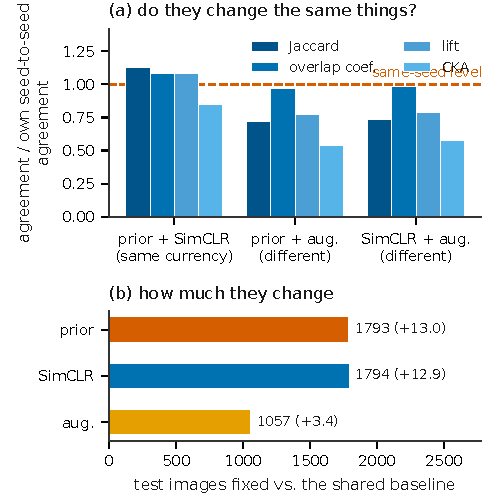
\includegraphics[width=\linewidth]{figs/currency_evidence.pdf}
\caption{Currency tested directly, not inferred from magnitudes.
All arms are ViT-tiny on CIFAR-100 at 10\% with one shared baseline, so
the only thing that varies is the fused source. \textbf{(a)} agreement
between two interventions in \emph{which} test images they fix and
\emph{which} representations they learn, each normalized by that
intervention's own seed-to-seed agreement, so $1.0$ means the two sources
differ no more than two seeds of one of them. Four measures are shown
because they do not agree on the size of the effect. \textbf{(b)} the
number of images each intervention fixes: the two same-currency sources
fix all but one the same number.}
\label{fig:currency}
\end{figure}
The prediction held on all four measures (Fig.~\ref{fig:currency}). The prior
and SimCLR fix $1793$ and $1794$ test images respectively, and their normalized
agreement on \emph{which} images is $1.13$ against $0.72$ for the prior with
augmentation; centred kernel alignment between their representations gives
$0.85$ against $0.53$. A value above one has a direct reading: for the question
of which images get fixed, it matters less whether you used a fixed spectral
target or contrastive pre-training than which seed you used. That is what a
substitute is.

Two qualifications. Augmentation fixes far fewer images ($1057$), and the
Jaccard measure penalizes a small set for being small; on the size-robust
overlap coefficient the separation shrinks to $1.08$ against $0.97$, so part of
the headline gap is a magnitude effect and only the representation-level
measure separates the pairs decisively. And this is one cell on one backbone;
it corroborates the taxonomy where the taxonomy already had its strongest
end-to-end evidence, instead of testing it somewhere new.

\emph{Takeaway.} What a source is worth depends on which currency is scarce,
not on how modern the source is: the same free prior is the most valuable
intervention we measure on an augmented ViT and the most damaging one on an
ImageNet-initialized ResNet.

%% ---------------------------------------------------------------------
\section{Validation at scale}\label{sec:scale}

Everything above could, in principle, have been a small-image regularity. We
therefore pre-registered a falsifier block and bought the two scale axes
separately: ImageNet64 (1.28M images, 1000 classes, 64\,px, 13$\times$ the
images and 5$\times$ the label space of anything else in the grid) and
ImageNet-100 at native $224$\,px with a model-scale curve (ViT-S/16, ViT-B/16,
ResNet-50, the ViTs under the standard DeiT recipe). Deviations (reduced
epochs; native-resolution transforms) apply equally to both arms of every pair.

\begin{table}[pos=htbp]
\caption{The pre-registered scale block. Every falsifier was declared
before the first run and none fired, with three qualifications kept in
view: ViT-S's $G$ landed $0.05$ below its registered band; ViT-B's
$|\Delta-G|$ of $3.12$ exceeds the registered $1.5$, on a cell whose
evaluation-ceiling limitation was also registered in advance and whose
residual is unresolvable; and
ResNet-50's $G$, registered at $-0.7$ to $-0.2$, measured $+0.19$, a $0.39$
miss across zero on a quantity that is a measured zero either way
($|\Delta - G| = 0.21$). $G$ at ImageNet64 uses the
fixed-budget evaluation (250 per class shown); ImageNet-100 the standard
full-train evaluation. Three seeds per cell; the
ImageNet-100 cells run $100$ epochs, and the text repeats both ViT pairs at
$200$, where the gains are $+4.52 \pm 0.18$ and $+6.71 \pm 0.90$.}
\label{tab:scale}
\centering\scriptsize
\setlength{\tabcolsep}{1.8pt}
\zebra{2}
\begin{tabular}{P{0.160\columnwidth}P{0.165\columnwidth}rrrP{0.145\columnwidth}}
\toprule
Cell & Registered band & $\Delta$~\up & $G$~\up & $|\Delta{-}G|$~\down & Verdict \\
\midrule
\multicolumn{6}{@{}l}{\emph{ImageNet64: 1.28M images, 1000 classes}} \\
ResNet-18 & $\Delta$: $0.0{\pm}0.5$ & $+0.04$\sem{0.08} & $+0.05$ & $0.01$ & neutral, exactly \\
MobileNetV3 & (none: in bracket) & $+1.95$\sem{0.40} & $+1.81$ & $0.14$ & consistent \\
ViT-tiny & $\Delta \geq +3$ & $+3.24$\sem{0.84} & $+2.84$ & $0.40$ & deficit persists \\
Swin-T &--& \multicolumn{3}{l}{baseline collapses at chance} & stabilized by prior \\
\midrule
\multicolumn{6}{@{}l}{\emph{ImageNet-100 @ 224\,px, DeiT recipe on ViTs}} \\
ResNet-50 & $\Delta$: $0.0{\pm}1.0$ & $-0.02$\sem{0.26} & $+0.19$ & $0.21$ & neutral at 224\,px \\
ViT-S/16 & $\Delta$: $+2..{+}8$; $G$: $12.0..12.6$ & $+13.00$\sem{0.24} & $+11.95$ & $1.05$ & above band \\
ViT-B/16 & $\Delta \geq \Delta_{\mathrm{ViT\mbox{-}S}}$ & $+26.01$\sem{2.01} & $+22.89^{*}$ & $3.12^{*}$ & grows at full data \\
\bottomrule
\rowcolor{white}\multicolumn{6}{@{}p{0.95\linewidth}@{}}{\footnotesize $^{*}$The ViT-B
aux arm evaluates at its own ceiling ($69.8$ vs.\ e2e $69.3$), a
pre-registered limitation that compresses $G$; the residual is not resolvable
against its uncertainty ($\pm 2.4$).} \\
\end{tabular}
\end{table}

Table~\ref{tab:scale} reports the block. Three conclusions.

\emph{Convolutional redundancy at sufficiency is exact and scale-stable.}
ResNet-18 at 1.28M images gains $+0.04 \pm 0.08$ end-to-end and $+0.05 \pm
0.10$ feature-side; the neutral regime measured to a hundredth of a point at
the largest data scale in the study. ResNet-50 at native $224$\,px repeats it:
the seed-paired difference on three matched seeds is $-0.02
\pm 0.26$, inside the pre-registered band ($0.0 \pm 1.0$), and the falsifier
that would have made convolutional redundancy
a low-resolution artifact ($\Delta \geq +1.5$) is ruled out.

\emph{The attention deficit is real, persistent, and grows with model scale at
full data.} ViT-tiny still gains $+3.2$ points at 1.28M images. At $224$\,px
under the standard recipe and a shared $100$-epoch budget, ViT-S/16 gains
$+13.0$ at $21.7$M parameters on a properly configured transformer, and
ViT-B/16 gains $+26.0$, twice ViT-S (the paragraphs below repeat both at a
doubled budget, where the ordering holds),
with the baseline's seed
variance three times the prior arm's. That asymmetry invites the obvious
objection, that the gain is the optimization stabilization
Sec.~\ref{abl:stab} treats as a separate property, so we settle it on the
seeds, not the standard deviation: the ViT-B baseline runs $46.5$, $39.9$ and
$43.6$, none of them near the $1\%$ chance level, so the cell does not trip the
collapse rule of Sec.~\ref{sec:stats}, and the \emph{worst} prior seed still
beats the \emph{best} baseline seed by $22$ points. Nothing here is a rescued
run. The pre-registered fork read: if the deficit is data-hunger, the bigger
model should show the larger gain. At full data it does, by 13 points. Notably,
at this budget and data scale the \emph{smaller} ViT with the prior still
outperforms the bigger one ($78.4$ vs.\ $69.3$): right-sizing plus structure
beats scale. Both are $100$-epoch numbers; at the doubled budget below, this
ordering also holds ($83.99$ against $82.02$).

\looseness=-1 That ordering was registered as a prediction across the whole envelope, not
only at full data: we recorded $\Delta_{\mathrm{ViT\text{-}B}} >
\Delta_{\mathrm{ViT\text{-}S}}$ \emph{at every fraction}, with a falsifier if
it inverted at any fraction at or above $5\%$. It inverts at $5$, $10$ and
$25\%$ (Table~\ref{tab:inenv}), so that falsifier fired and we report it (it
also inverts nominally, unresolved, at $1$ and $2\%$). We do
not read those cells as refuting the full-data result, and the reason is a
property of the arms themselves. Below $100\%$ the ImageNet-100 ViT-B baseline
never trains, flat at $4.1$--$7.1\%$ on a 100-way task across a $12.5\times$
data range, so its gain there cannot carry a claim about model scale; and the
comparator arm, ViT-S, carries baseline seed standard deviations up to $8.2$
points at exactly the fractions ($10$ and $25\%$) where it produces the
larger gain driving the inversion. The defensible claim is
the narrower one: at full data the deficit
grows with model scale, and across the low-data fractions of this population
the comparison is not determined.

\paragraph{Is the ViT-B gain an under-trained baseline?} The $+26.01$ is the
largest number in this paper and it is measured at $100$ epochs, where an
85.9M-parameter transformer on $126$k images may not have finished training. We
doubled the schedule on both arms, six seeds each.
The baseline gains $+31.98$ from the schedule alone, reaching $75.31 \pm 0.48$;
the prior arm reaches $82.02 \pm 0.76$; the gain is $+6.71 \pm 0.90$, $95\%$
confidence interval $[4.94, 8.47]$, $7.4$ standard errors from zero. About a
quarter of the headline survives a doubled schedule, so $+26.01$ is a
$100$-epoch figure and should be read with $+6.71$ beside it.

\looseness=-1 We had registered a falsifier at $\Delta \leq +6$, which would have withdrawn
the model-scale conclusion outright. The interval contains $6.0$, which sits
$0.78$ standard errors below the estimate, so the falsifier is neither fired
nor excluded and we report it as exactly that. Two facts belong beside it. The
estimate moved with seeds, $+7.79$ at three arms against two, $+7.79$ at three
against three and $+6.71$ at six against six, so a three-seed report would have
published a clearance the data do not support. And one prior-arm seed, $78.58$,
sits $4.6$ standard deviations below the other five ($82.71 \pm 0.90$); it is
not a collapse under the rule of Sec.~\ref{sec:stats} and there is no
principled reason to drop it, so it stays, and it is why this arm's uncertainty
exceeds the baseline's. Excluding it would give $+7.39 \pm 0.63$ and put the
threshold outside the interval, which is exactly why we keep it.

\paragraph{The trend at a budget where both models are trained.} The
comparison motivating that trend, $+13.00$ against $+26.01$, is made at $100$ epochs,
where the control above shows ViT-B still $+31.98$ short of where the schedule
alone takes it, so we repeated ViT-S at $200$ epochs too, six seeds per arm.
It reaches $79.47 \pm 0.16$ against $83.99 \pm 0.08$, a gain of $+4.52 \pm
0.18$, against ViT-B's $+6.71 \pm 0.90$. The ordering holds by $-2.19 \pm
0.92$, and the pre-registered falsifier, which would have withdrawn the
model-scale claim everywhere had ViT-S matched or exceeded ViT-B, did not fire.
The uncertainty is almost entirely ViT-B's (standard errors $0.48$ and $0.76$
against ViT-S's $0.16$ and $0.08$), so the ordering is clear at $2.4$ standard
errors and not tighter. We tested it expecting it to invert.

\emph{The law's predictive form survives.} Five of six pairs tie $\Delta$ to
$G$ within $1.1$ points; the sixth (ViT-B) carries a pre-registered
evaluation-ceiling limitation and an unresolvable residual. That ceiling
caveat belongs to every ImageNet-100 row, not to ViT-B alone: at these
$100\%$ cells the evaluation's labels are the cell's own, so the
$|\Delta - G|$ column is a gap read under the scope rule of
Sec.~\ref{sec:probe}, not a signed \readout{}, which is why the cells stand
here and not in the audit of Sec.~\ref{sec:lawaudit}; the ImageNet64
rows, evaluated at fixed per-class budgets, carry no ceiling. The ViT-S band,
derived from the law before the evaluation ran, was hit on its edge ($11.95$
vs.\ $12.0$--$12.6$). As an additional robustness check, the ViT-S and
ResNet-50 evaluations were independently re-run on a second machine with a
from-scratch environment; their means agree with the primary measurement to
$0.01$--$0.05$ points.

\subsection{The envelope at ImageNet scale}\label{sec:scaleenvelope}

The block above measures the right-hand end of the envelope. Because that would
leave the shape untested at scale, both ImageNet stages were also run across
fractions, on the same fixed subsets and the same reduced-epoch budget as their
$100\%$ cells (Table~\ref{tab:inenv}). This is the largest data-efficiency
envelope in the study, and it reports a registered miss before it reports
anything else.

\emph{The miss.} We registered an interior peak at $5$--$20\%$ for the
convolutional envelope. ResNet-18 instead falls from the smallest
runnable fraction, $+1.90$ at $1\%$ to zero by $10$--$15\%$, staying within
$0.2$ of zero thereafter, with no interior peak:
the falsifier fired. The cause is that we predicted in \emph{fraction} space
when the operative axis is absolute data. One percent of ImageNet64 is
$12{,}820$ images, which on every smaller population in the grid is already
past the peak. The envelope is not absent at scale; its peak sits below the
smallest fraction this dataset can express.

\emph{What the same cells then show, which we did not anticipate.} Holding
dataset, recipe, subsets and label space fixed and varying only the backbone
gives three different envelope shapes (Fig.~\ref{fig:inenv}). ResNet-18 falls
to zero and stays there; ViT-tiny and MobileNetV3 rise monotonically across the
entire measured range, ViT-tiny from $+2.14$ to $+7.75$ at $25\%$. Under the
account this is not three phenomena but one: the peak sits where the baseline
crosses the \readout{} bracket, and only ResNet-18's baseline reaches it in range
($5.5 \to 47.2$, crossing $[31.8,40.3]$ between $7$ and $15\%$), which is
exactly where its gain reaches zero ($+0.42$ at base $32.3$, $-0.01$ at base
$42.3$). Across $1$--$25\%$ neither of the others comes near the band and both
are still climbing; extend to full data and they arrive too, MobileNetV3 into
it ($32.9$) and ViT-tiny above it ($48.2$), and both gains duly fall ($+3.45
\to +1.95$ and $+7.75 \to +3.24$). One rule, three apparent shapes: the
envelope's peak is a property of where a \emph{backbone} sits on its own
\readout{} curve, not of the dataset, and this is the cleanest demonstration of
that in the paper, because the classification grid could only vary it by
changing datasets too.

\begin{figure}[pos=htbp]
\centering
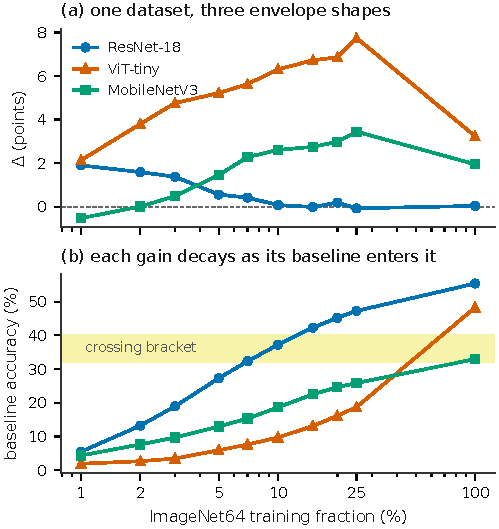
\includegraphics[width=\linewidth]{figs/inenv.pdf}
\caption{The envelope at ImageNet scale, and why its shape is a property of
the backbone. Dataset, recipe, fixed subsets and label space are held
constant; only the backbone varies. \textbf{(a)} Three backbones, three
envelope shapes: ResNet-18 falls to zero and stays there, while ViT-tiny and
MobileNetV3 climb across the whole range. \textbf{(b)} The same baselines
against the crossing bracket. Each gain decays as its own baseline enters the
band, and the three arrive at very different fractions: ResNet-18 by
$7$--$15\%$, MobileNetV3 only at $100\%$, ViT-tiny passing above it at
$100\%$, exactly where its gain falls. Three seeds per cell.}
\label{fig:inenv}
\end{figure}

\begin{table}[pos=htbp]
\caption{The envelope at ImageNet scale: $\Delta$ by fraction, three seeds
per cell, both arms sharing the reduced-epoch budget. Baseline accuracy is
given beneath each gain. ImageNet64's three backbones see identical images,
recipe and label space, so the difference in envelope \emph{shape} between
them is attributable to the backbone alone. The ImageNet-100 ViT columns
below $100\%$ are reported with a caveat, not as headline cells:
their baselines sit close to chance and carry seed standard deviations up to
$8.2$ points, so the gains there are large but poorly determined. Every
ImageNet-100 cell here uses the $100$-epoch budget; the ViT-B pair at $200$
epochs gives $+6.71$ (Sec.~\ref{sec:scale}). Best in bold and second best
underlined, per fraction within each stage; with three backbones per stage the
remaining entry is third, so no italic mark is needed.}
\label{tab:inenv}
\centering\scriptsize
\setlength{\tabcolsep}{2.2pt}
\zebra{5}
\begin{tabular}{lrrrrrr}
\toprule
& \multicolumn{3}{c}{ImageNet64, 64\,px} & \multicolumn{3}{c}{ImageNet-100, 224\,px} \\
\cmidrule(r){2-4}\cmidrule(l){5-7}
Frac. & R18 & ViT-Ti & MNetV3 & R50 & ViT-S & ViT-B \\
\midrule
1\%   & \snd{$+1.90$} & $\mathbf{+2.14}$ & $-0.52$ & $+0.54$ & $\mathbf{+2.31}$  & \snd{$+0.69$} \\
      & \tiny 5.5 & \tiny 1.9 & \tiny 4.3 & \tiny 11.5 & \tiny 7.3 & \tiny 5.3 \\
2\%   & \snd{$+1.59$} & $\mathbf{+3.80}$ & $+0.01$ & $+1.21$ & $\mathbf{+7.59}$  & \snd{$+5.11$} \\
      & \tiny 13.2 & \tiny 2.6 & \tiny 7.6 & \tiny 18.2 & \tiny 6.4 & \tiny 4.1 \\
3\%   & \snd{$+1.38$} & $\mathbf{+4.76}$ & $+0.49$ &--&--&-- \\
      & \tiny 18.9 & \tiny 3.4 & \tiny 9.7 &&& \\
5\%   & $+0.56$ & $\mathbf{+5.22}$ & \snd{$+1.46$} & $+1.84$ & $\mathbf{+14.15}$ & \snd{$+4.47$} \\
      & \tiny 27.3 & \tiny 5.9 & \tiny 12.9 & \tiny 36.5 & \tiny 7.3 & \tiny 6.1 \\
7\%   & $+0.42$ & $\mathbf{+5.63}$ & \snd{$+2.28$} &--&--&-- \\
      & \tiny 32.3 & \tiny 7.6 & \tiny 15.3 &&& \\
10\%  & $+0.08$ & $\mathbf{+6.31}$ & \snd{$+2.61$} & $+1.74$ & $\mathbf{+14.23}$ & \snd{$+2.30$} \\
      & \tiny 37.2 & \tiny 9.7 & \tiny 18.6 & \tiny 55.7 & \tiny 11.9 & \tiny 6.6 \\
15\%  & $-0.01$ & $\mathbf{+6.72}$ & \snd{$+2.75$} &--&--&-- \\
      & \tiny 42.3 & \tiny 13.1 & \tiny 22.5 &&& \\
20\%  & $+0.19$ & $\mathbf{+6.86}$ & \snd{$+2.98$} &--&--&-- \\
      & \tiny 45.2 & \tiny 16.1 & \tiny 24.6 &&& \\
25\%  & $-0.07$ & $\mathbf{+7.75}$ & \snd{$+3.45$} & $+2.30$ & $\mathbf{+30.39}$ & \snd{$+7.36$} \\
      & \tiny 47.2 & \tiny 18.7 & \tiny 25.8 & \tiny 72.5 & \tiny 23.2 & \tiny 7.1 \\
100\% & $+0.04$ & $\mathbf{+3.24}$ & \snd{$+1.95$} & $-0.02$ & \snd{$+13.00$} & $\mathbf{+26.01}$ \\
      & \tiny 55.4 & \tiny 48.2 & \tiny 32.9 & \tiny 85.9 & \tiny 65.4 & \tiny 43.3 \\
\bottomrule
\end{tabular}
\end{table}

\looseness=-1 Two further readings. The convolutional column reaches sufficiency inside the
measured range and stays there, so the neutrality result of
Table~\ref{tab:scale} is not a single point but a plateau from $10\%$ of
ImageNet64 onward. And ResNet-50 at $224$\,px is the one convolutional column
that is \emph{positive} in the low-data band ($+0.5$ to $+2.3$ from 1 to
$25\%$) before returning to neutrality at full data. We had registered $+1$ to
$+6$ across 1--5\% with a decay through $25\%$, and both halves missed: the
$1\%$ cell lands at $+0.54$, below the band, and the column rises instead of
decaying ($+1.74$ at $10\%$, $+2.30$ at $25\%$). What held is the direction and
the falsifier, which would have fired had $\Delta$ been non-positive
everywhere: convolutional gains do survive native resolution and are a
low-data, not a low-resolution, phenomenon, but we did not call their size or
their shape.

\emph{Takeaway.} Scale does not retire the prior: convolutional redundancy at
sufficiency survives 1.28M images, while attention's deficit grows with model
size, not shrinking. Filling the envelope at scale cost us a registered
prediction and returned a sharper claim in its place: which fraction the peak
sits at is a property of the backbone's position on the \readout{} curve, not of
the dataset.

%% ---------------------------------------------------------------------
\section{Buying the comparator more compute}\label{sec:budget}

\looseness=-1 Cost normalization makes the comparisons in Sec.~\ref{sec:law}
interpretable, and Sec.~\ref{sec:parity} states its price: a comparator held
to its published budget inside our recipe may be undertrained, not weak, and
the two are not separable by construction. We measured that reservation rather
than leave it as a limitation, re-running both self-supervised comparators at
four times their pre-training budget and at every fraction from 1 to 25\%,
since every other effect here moves with the data regime.
Table~\ref{tab:budget} reports it, and
Secs.~\ref{sec:budget:simsiam}--\ref{sec:budget:features} work through it.
The objection is confirmed outright: it costs us an accuracy claim on
convolutional backbones, attaches a budget and a data regime to the claim that
survives on attention, and replaces one account of our two populations'
difference with another.

\begin{table}[pos=htbp]
\caption{Buying the comparators more compute. CIFAR-100, ResNet-18, gain
over the baseline by data fraction; three seeds per pre-trained cell, ten
for the baseline and the prior at 1, 5 and 10\%. SSm is SimSiam and SC is
SimCLR, at 200 pre-training epochs ($2\times$ baseline compute) or 800
($5\times$); the prior costs $1.02\times$. The last two columns give the
prior minus each $5\times$ comparator, where positive
means the free prior still wins.}
\label{tab:budget}
\centering\scriptsize
\setlength{\tabcolsep}{2.6pt}
\zebra{6}
\begin{tabular}{lrrrrrrr}
\toprule
 & \textbf{Prior} & \multicolumn{2}{c}{$2\times$ SSL} & \multicolumn{2}{c}{$5\times$ SSL} & \multicolumn{2}{c}{prior $-$ $5\times$} \\
\cmidrule(lr){3-4}\cmidrule(lr){5-6}\cmidrule(l){7-8}
Frac. & $\mathbf{1.02\times}$~\up & SSm~\up & SC~\up & SSm~\up & SC~\up & SSm & SC \\
\midrule
1\%  & $+1.42$ & $-0.02$ & $+2.27$ & $-0.09$ & $\mathbf{+4.54}$ & $+1.51$ & $-3.12$ \\
2\%  & $+2.50$ & $-0.11$ & $+4.88$ & $+0.19$ & $\mathbf{+8.33}$ & $+2.31$ & $-5.83$ \\
3\%  & $+3.68$ & $+0.11$ & $+5.99$ & $+0.54$ & $\mathbf{+10.82}$ & $+3.14$ & $-7.14$ \\
5\%  & $+5.15$ & $+0.13$ & $+9.05$ & $+1.90$ & $\mathbf{+14.38}$ & $+3.25$ & $-9.23$ \\
7\%  & $+4.87$ & $+0.87$ & $+9.86$ & $+3.39$ & $\mathbf{+13.88}$ & $+1.48$ & $-9.01$ \\
10\% & $+3.75$ & $+0.61$ & $+8.76$ & $\mathbf{+4.33}$ & $\mathbf{+10.92}$ & $-0.58$ & $-7.17$ \\
15\% & $+2.55$ & $+0.17$ & $+6.64$ & $+3.65$ & $\mathbf{+8.36}$ & $-1.10$ & $-5.81$ \\
25\% & $+0.16$ & $-0.03$ & $+2.81$ & $+0.79$ & $\mathbf{+2.77}$ & $-0.63$ & $-2.61$ \\
\bottomrule
\end{tabular}
\end{table}

\subsection{The near-null was a budget artifact}\label{sec:budget:simsiam}
SimSiam at its published 200-epoch budget gains nothing anywhere on the
envelope, $-0.11$ to $+0.87$. At 800 epochs it gains up to $+4.33$. We
therefore withdraw the statement that negative-free self-supervision learns
almost nothing at this scale: it is budget-starved at the cost we normalized
to, and its published default is a poor guide to what it can do on a few
thousand images. Its budget response is itself data-dependent, \looseness=-1
buying most in the mid band ($+3.7$ at 10\%) and nothing at 1\%.

That data-dependence is why the envelope was necessary. The full
envelope shows a crossover: the prior wins from 1 to 7\% by up to $3.25$ ($2.6$
to $12.2$ standard errors) and \emph{loses} from 10 to 25\%, most clearly at
15\% ($-1.10$, $5.2$). A read at 5 and 10\% alone, where the objection is
sharpest, would have missed a significant
reversal, the same sparse-grid error we identify in our own earlier readings.

\subsection{On convolutions the prior's case becomes a cost
case}\label{sec:budget:conv} Against the stronger comparator the prior loses at
every fraction, including the scarcest. SimCLR at $5\times$ beats it by $3.12$
to $9.23$ points, at 12 to 37 standard errors, from 500 images to 7{,}500
(1--15\%), and by a narrowing $2.61$ at 25\% as both interventions decay toward
sufficiency. Our earlier positioning noted near-parity with self-supervision at
1\%; that was a statement at $2\times$ and it does not survive $5\times$. On
convolutional backbones the prior's case is therefore a cost case and not an
accuracy case, and we say so without qualification.

\subsection{Attention, given the same test}\label{sec:budget:vit}
Leaving the attention comparison at $2\times$ while raising the convolutional
one to $5\times$ would reproduce exactly the asymmetry this section exists to
remove, so we ran it there too. Against ViT-tiny under the DeiT recipe,
$5\times$ SimCLR gives $30.45$, $40.57$ and $55.85$ at 5, 10 and 25\%, against
the prior's $28.87$, $41.29$ and $57.32$. The comparator \emph{wins} at 5\% by
$1.57$ ($3.9$ standard errors, six seeds), the two are level at 10\% ($+0.71$,
$1.2$), and the prior wins at 25\% by $1.47$ ($7.2$). The prior is not
overturned on attention as it is on convolutions, but the claim must name its
budget: at $2\times$ the prior leads at every CIFAR-100 fraction, and at
$5\times$ only in the higher-data band. Section~\ref{sec:budget:tin} shows the same boundary
on a second population.

That shape contradicted a prediction recorded before the runs: we expected the
prior to hold at the scarce fractions and 25\% to be the cell most likely to
flip, and the reverse happened. What the extra budget buys shows why: $+8.80$,
$+4.51$ and $+3.53$ at 5, 10 and 25\%, decreasing with data, because 200 epochs
over 2{,}500 images is fewer than four thousand steps: the comparator was
step-starved at 5\%, not data-starved (Sec.~\ref{sec:dataopt}). On
convolutional backbones the same increment peaks in the mid band, so the budget
response is itself backbone-dependent.

\subsection{A second population, and the account that
failed}\label{sec:budget:tin} Repeating the comparison on Tiny-ImageNet gives
the same ordering at every matched fraction. Writing the prior minus a
$5\times$-budget SimCLR initialization, both under DeiT augmentation on
ViT-tiny, CIFAR-100 gives $-1.57$, $+0.71$ and $+1.47$ at 5, 10 and 25\%, and
Tiny-ImageNet gives $-1.35$, $-0.31$ and $+1.71$. The comparator wins at 5\% on
both ($3.9$ and $3.7$ standard errors), the two are level at 10\% on both, and
the prior wins at 25\% on both ($7.2$ and $5.1$). So at five times the
comparator's pre-training budget the prior leads in the higher-data band and
loses in the scarcer one, and that pattern is not specific to a dataset. The
ordering tracks the data fraction, not the absolute image count: $5{,}000$
images is 10\% of CIFAR-100 but 5\% of Tiny-ImageNet, and the two disagree
there while agreeing at every matched fraction.

Getting there cost us a prediction and an account. With only the 5 and 10\%
cells measured, where the comparator was ahead and level, we wrote that the
prior led nowhere on this population, predicted the 25\% cell at $40$--$44$
explicitly against our own method, and expected the two populations to line
up by image count. The cell landed at $36.53$, below the band; the recorded
falsifier fired; and the matched-fraction table shows why the account was
wrong: matching on image count compares different points on two different
learning curves, and what determines which source wins is where a cell sits
on its own dataset's curve. The ``different stories'' reading was an
artifact of a two-point grid, the same error this section has already
documented once.

One measurement in this pass we report without explaining. At Tiny-ImageNet
25\%, four times the pre-training made the comparator \emph{worse}: $38.48$ at
$2\times$ against $36.53$ at $5\times$, a drop of $1.95 \pm 0.42$. It is the
only cell in the study where extra pre-training budget costs accuracy, and it
echoes our earlier finding that DeiT-strength contrastive views also hurt. We
note it and decline to fit an explanation to one cell.

\subsection{What the budget actually buys}\label{sec:budget:features}
The comparison so far is end-to-end, while the taxonomy is a claim about
\emph{what} a source supplies, not how much accuracy it yields, so we
probed these cells under the frozen-feature protocol used throughout.

On CIFAR-100 the feature gain of $5\times$ SimCLR is $+22.24$, $+21.27$ and
$+20.77$ at 5, 10 and 25\%, against the prior's $+21.37$, $+22.19$ and
$+23.05$. The two orderings agree cell by cell: the comparator's feature gain
is larger where it wins end-to-end, level where the two are level, and smaller
where the prior wins. The prior's feature gain \emph{rises} with data while the
comparator's \emph{falls}, and they cross between 5 and 10\%, which is where
the accuracy ordering crosses. Extra pre-training budget therefore buys more of
the same currency, not a different one, and the flip is a property of the
representations, not of the classifier reading them. This is the substitution
outcome measured on a budget axis, the one axis the taxonomy had not been
tested on.

\looseness=-1 Including the second population strengthens the agreement and supplies the
mechanism the image-count account lacked. Across both datasets and all six
measured fractions, whichever intervention has the larger frozen-feature gain
wins end-to-end: the sign of $G_{\mathrm{SSL}} - G_{\mathrm{prior}}$ matches
the sign of the accuracy difference six times out of six. The clearest case is
the cell that overturned our own prediction. At Tiny-ImageNet 25\%, where the
prior wins by $1.71$, its feature gain is $+14.27$ against the comparator's
$+12.43$; that difference of $1.84$ agrees with the accuracy difference to
within $0.13$, so the outcome is feature-side almost entirely. The population
term is equally unmysterious once measured. At a matched 5{,}000 images the two
datasets diverge because the \emph{prior's} contribution diverges: its feature
gain is $+22.19$ on CIFAR-100 against $+15.67$ on Tiny-ImageNet, while the
comparator's is $+21.27$ and $+17.72$. Moving to the 200-way $64$\,px task
costs contrastive pre-training about $3.5$ points of feature gain and the fixed
spectral target about $6.5$: the hand-crafted prior supplies proportionally
less of what a finer label space at higher resolution requires, and that,
not the number of images, decides which source wins.\footnote{The
Tiny-ImageNet comparator probes were computed on a different machine from the
cells they pair with. Cross-machine agreement under this protocol was verified
elsewhere in the study to within $0.05$ points, but we note the mixed
provenance instead of leaving it implicit.}

The second comparator extends the same agreement. Probing SimSiam at $5\times$
across all eight fractions gives a feature gain that sits below the prior's
from 1 to 7\% ($-5.3$ to $-1.9$ points of difference), crosses at 10\%, and
rises above it at 15\%, matching the end-to-end ordering reported in
Sec.~\ref{sec:budget:simsiam} at seven of eight cells; the one mismatch is
the crossing cell itself, where the feature difference is a near-zero $-0.08$. Across two
self-supervised methods and two backbone families, the source with the larger
frozen-feature gain is the one that wins.

\looseness=-1 One result in this pass we report without an account. Probing the convolutional
budget envelope shows the prior's own residual tracking the fitted branch
closely ($-2.74$, $-2.65$, $-2.07$, $-1.11$ below the crossing, $+0.06$ and
$+0.21$ inside the bracket, and $-0.18$, $-0.28$ above it), while $5\times$ SimCLR departs from it,
running positive from 3 to 15\% ($+1.32$, $+3.11$, $+3.58$, $+2.23$, $+1.81$)
at baselines where the branch is negative or near zero. Two things narrow what
the anomaly can be. It is not a property of self-supervised initialization as
such: $5\times$ SimSiam, initialized the same way and evaluated identically,
stays within $[-0.42, +0.86]$ at every fraction. And across all sixteen
self-supervised convolutional cells the residual correlates with the size of
the intervention itself ($r = +0.52$ between $\Delta$ and the residual), so
what departs from the branch is large gains rather than a particular method. We
recorded in advance that these initializations lie outside the scope in which
the branch was estimated, so we do not count the departure against it, and we
prefer to leave it as a measured regularity than to fit an explanation to
sixteen points.

\emph{Takeaway.} A comparator's budget is part of the claim. Two of our own
accuracy claims did not survive this section and are now cost claims; the
finding that did survive is that heavy augmentation, not the prior, is what
collapses contrastive pre-training's advantage.

%% ---------------------------------------------------------------------
\section{Fusing genuinely different sources}\label{sec:multisource}

Everything to this point fuses one knowledge source into one image stream.
This section asks whether the same rule governs fusion in the sense the
term usually carries: two \emph{sensors}, and two \emph{classifiers}.
Section~\ref{sec:multisensor} takes visible and non-visible Sentinel-2
bands as separate sources; Section~\ref{sec:decisionfusion} fuses trained
models at the decision level. Both are tests of transfer rather than
restatements: the rule was derived from training-time fusion of a prior
into a network, and neither of these is that.

\subsection{Two sensors: multispectral EuroSAT}\label{sec:multisensor}
EuroSAT ships as 13 Sentinel-2 bands, of which three are visible. The
visible bands and the red-edge, near-infrared, short-wave infrared and
cirrus bands come from different detectors and carry different physical
information, which makes the complementary-versus-redundant question
askable of the data itself. We build three sources from one archive:
\textbf{visible} (3 bands), \textbf{non-visible} (the other 10), and
\textbf{sensor-fused} (all 13). The tiles and the committed subset indices
are identical across the three, so the only thing that varies is which
detectors the network reads. Each is crossed with the baseline and the
prior under the frozen recipe.

\begin{table}[t]
\caption{Multispectral EuroSAT. Identical tiles and identical subset
indices; only the band set differs. Three seeds per cell, ResNet-18. The
prior's gain \emph{grows} with the number of sensors present rather than
being absorbed by them, and the same ordering appears in the frozen-feature
evaluation, so it is a feature-level effect.}
\label{tab:sensorfusion}
\centering\scriptsize
\setlength{\tabcolsep}{2.6pt}
\zebra{2}
\begin{tabular}{@{}P{0.26\columnwidth}rrrr@{}}
\toprule
Source & Baseline~\up & + Prior~\up & $\Delta$~\up & $G$~\up \\
\midrule
\multicolumn{5}{@{}l}{\emph{5\% of the training split (1{,}080 tiles)}} \\
Visible (3 bands) & 89.56 & 91.19 & $+1.63$ & -- \\
Non-visible (10) & 90.14 & 92.73 & $+2.60$ & -- \\
Sensor-fused (13) & \textbf{91.48} & \textbf{94.78} & $\mathbf{+3.30}$ & -- \\
\midrule
\multicolumn{5}{@{}l}{\emph{25\% of the training split}} \\
Visible (3 bands) & 97.88 & 97.85 & $-0.02$ & $-0.02$ \\
Non-visible (10) & 97.77 & 98.19 & $+0.43$ & $+0.28$ \\
Sensor-fused (13) & \textbf{98.33} & \textbf{98.65} & $+0.33$ & $+0.37$ \\
\bottomrule
\end{tabular}
\end{table}

Table~\ref{tab:sensorfusion} reports three things.

\emph{The two band sets are complementary.} Fusing them beats the better
single sensor by $+1.34$ at 5\%, $+1.15$ at 10\% and $+0.45$ at 25\%. This
is the stack outcome, measured on the data rather than on a training
intervention, and it decays with data exactly as every other effect in this
study does: by 25\% of a 21{,}600-tile archive there is little left for a
second sensor to contribute.

\emph{The prior's gain grows with the number of sensors.} At 5\% it is
$+1.63$ on the visible bands, $+2.60$ on the non-visible, and $+3.30$ on
both. Had oriented-energy structure been a substitute for spectral
coverage, adding detectors would have absorbed it; instead the two
compound. This is the sharpest available statement of the currency account,
because the second source here is a physical sensor rather than another
training trick, and its currency is unambiguously not the prior's.

\emph{And it is a feature-level effect.} Under identical frozen-feature
evaluation, $G$ moves in the same order as $\Delta$: $-0.02$, $+0.28$,
$+0.37$. The law's arithmetic also holds where it should. All three
baselines sit near 98\%, far above the crossing bracket, where the account
predicts a readout term of ${\approx}0$; the measured residuals are
$0.00$, $+0.15$ and $-0.04$.

\subsection{Two classifiers: decision-level fusion}\label{sec:decisionfusion}
Multi-classifier fusion is a different level again, and the rule was not
derived there. Using trained checkpoints from the CIFAR-100 5\% cells and
no further training, we average class posteriors for every pair of arms and
record the gain over the better single arm together with the pair's
disagreement rate, the classical diversity measure
\citep{brown2005diversity}.

The first thing the data say is a caution rather than a confirmation.
Ensemble gain is well explained ($R^2 = 0.74$) by two terms, and the
dominant one is not diversity:
\begin{equation}
  \mathrm{gain} \;=\; -2.74 \;+\; 0.089\,\mathrm{disagreement}
                       \;-\; 0.341\,|\Delta_{\mathrm{acc}}| ,
  \label{eq:ensgain}
\end{equation}
so pairing a strong arm with a weak one destroys the gain regardless of
what either contributes. Restricting to pairs within one point of each
other, where currency is actually the free variable, leaves three:

\begin{center}\scriptsize
\begin{tabular}{@{}P{0.34\columnwidth}rr@{}}
\toprule
Pair & Gain~\up & Disagreement \\
\midrule
Prior + SimCLR (50 ep) & $+1.20$ & 47.2\% \\
SimCLR (50 ep) + prior, wide bank & $+1.13$ & 47.2\% \\
Prior + prior, wide bank & $-0.04$ & 28.1\% \\
\bottomrule
\end{tabular}
\end{center}

Two models built on the same knowledge source disagree on 28\% of test
images and ensembling them buys nothing; pair either with a
self-supervised model and disagreement rises to 47\% and ensembling buys
${\sim}1.2$ points. That is the currency rule with its mechanism visible,
and it is what the classical account would predict.

We report the qualification with equal weight, because it bounds the
taxonomy rather than extending it. The prior and SimCLR do \emph{not} stack
at training time (Section~\ref{sec:substitute}), yet they ensemble usefully
at decision time ($+1.24$). Redundancy in the sense of ``jointly training on
both adds nothing'' therefore does not imply redundancy in the sense of
``their errors are correlated''. The substitution result is a statement
about training-time fusion, and we do not claim it transfers to decision
fusion. With three matched pairs this is suggestive rather than
established, and we say so.

\subsection{A procedure for deciding whether to fuse}\label{sec:procedure}
The practical content of the taxonomy is that the outcome of a combination
can be estimated \emph{before} the combined system is built, from
measurements of each source alone. We state that as a procedure rather than
as a finding, since it is what a practitioner would actually run.

\begin{table}[t]
\caption{Deciding whether to fuse two sources, before training the
combination. Every quantity is measured on the sources separately; the only
cost beyond training each source once is two frozen-feature evaluations.}
\label{tab:procedure}
\centering\scriptsize
\setlength{\tabcolsep}{2.6pt}
\zebra{2}
\begin{tabular}{@{}P{0.05\columnwidth}P{0.86\columnwidth}@{}}
\toprule
\multicolumn{2}{@{}l}{\textbf{Inputs}: sources $A$, $B$; a baseline arm; a labelled split} \\
\midrule
1 & Train the baseline, $A$ alone and $B$ alone. Record each arm's
    end-to-end gain and declared compute multiple. \\
2 & Evaluate all three frozen representations with an identical linear
    protocol. This gives $G_A$ and $G_B$, each source's feature-level
    contribution. \\
3 & If either source's gain is ${\approx}0$, it supplies nothing to
    overlap: the other source's gain is available in full, and the
    combination is not the question. \\
4 & If $G_A \approx G_B$ \emph{and} both arms improve the same cells,
    the sources carry the same currency. Expect \textbf{substitution}:
    the combination will not exceed the better single arm. Take the
    cheaper source. \\
5 & If $G_A$ and $G_B$ differ in kind, expect \textbf{stacking}, and a
    combined gain larger than either alone. \\
6 & If one source is a mature initialization, do not inject a shaping
    prior on top of it. Expect a \textbf{tax} proportional to what the
    initialization was contributing, measurable in advance as that
    source's advantage over training from scratch. \\
\bottomrule
\end{tabular}
\end{table}

Table~\ref{tab:procedure} states it. Three properties are worth drawing
out. It is \emph{cheap}: the only cost beyond training each source once is
two linear evaluations on frozen features, which run in minutes on cells
that took hours to train. It is \emph{predictive rather than
retrospective}, which places it alongside transferability estimation
\citep{nguyen2020leep,you2021logme}, with the difference that those methods
score a single pre-trained source for a target task while this scores a
\emph{pair} for combination. And it is \emph{falsifiable}: step 4 asserts
that equal feature gains imply no benefit from combining, which
Sections~\ref{sec:substitute} and \ref{sec:decisionfusion} both test and
which the training-time-versus-decision-time discrepancy above already
qualifies.

The honest limit is step 4's antecedent. We compare feature gains by
magnitude and by which cells improve, not by a formal decomposition of the
information each source carries. Partial information decomposition
\citep{williams2010nonnegative,liang2023quantifying} is the principled
version of that comparison, and an estimator that scaled to these
representations would replace our proxy with a quantity that means
something on its own.

%% ---------------------------------------------------------------------
\section{Does any of this hold off classification?}\label{sec:dense}

Every number to this point is top-1 accuracy. That is a real limit on what
the benchmark can claim, since the auxiliary target is itself a \emph{dense}
map, oriented energy at every location, so a reader is entitled to ask
whether the fusion outcomes and the law $\Delta = G + \readout$ are
properties of the method or of the metric. This section answers that on
semantic segmentation, then on object detection, where the answer changes.

\textbf{State the bias before the result.} A dense spatial target on a dense
spatial task is the most favourable venue this prior could be given, so a
\emph{positive} result here would be weak evidence of generality; what makes
the experiment worth running is that its headline finding is negative, and
negatives are not flattered by a favourable venue.

\paragraph{Setup.} Six populations spanning label-space width and domain:
\textbf{PASCAL VOC-2012} (21 classes, augmented split), \textbf{Cityscapes}
(19, driving, half resolution), \textbf{FoodSeg103} (104, texture-dominated),
\textbf{ADE20K} (150, scene-centric, no background class),
\textbf{Pascal-Context} (254), and a \textbf{Swin-Tiny} arm on VOC. The encoder
is the study's ResNet-18 at output stride 8 with an FCN head, so the prior's
bank, tap, $\lambda$ schedule and head normalization transfer with no re-design
and no new hyper-parameter. Table~\ref{tab:dense} gives the full envelope and
Fig.~\ref{fig:dense} summarises it. \densePops{} populations $\times$ six
fractions $\times$ two arms $\times$ three seeds $=$ \denseCells{} runs (72
cells in the sense of Sec.~\ref{sec:stats}), all completed.

\begin{figure}[pos=htbp]
\centering
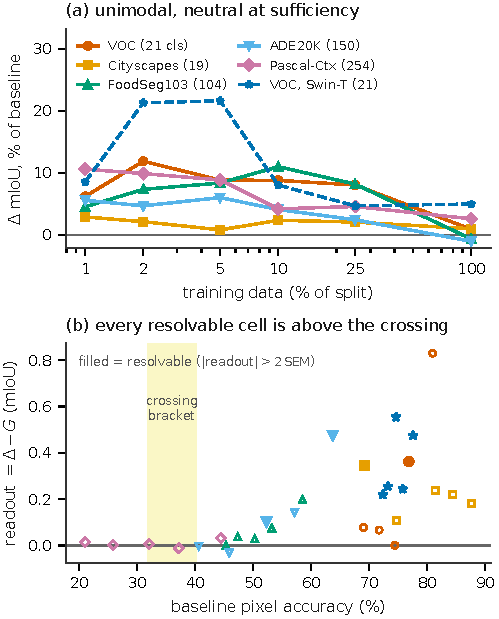
\includegraphics[width=\linewidth]{figs/dense_envelope.pdf}
\caption{Semantic segmentation, six populations, 200 epochs, three seeds per
cell. \textbf{(a)} $\Delta$ as a percentage of each cell's own baseline, not absolute mIoU, since the baselines differ eightfold. Read this way, four of
the six envelopes are unimodal, Cityscapes is flat within noise and
Pascal-Context is highest at $1\%$ and lower everywhere after; all six occupy
the same \denseRelLo--\denseRelHi\% band classification does across
$1$--$25\%$, and three go neutral or
negative at full data. \textbf{(b)} The \readout{} term against the head's own classification scale
(pixel accuracy), not mIoU: the crossing bracket is an accuracy bracket, and
scoring the law on mIoU puts every dense cell on the wrong flank. Filled
markers are the resolvable cells; all sit above the bracket, so segmentation
confirms the law's positive branch and cannot test its negative one.}
\label{fig:dense}
\end{figure}


Pascal-Context is the control that carries most of the weight: it re-annotates
the \emph{identical} VOC images at 254 classes instead of 21, so it separates a
label-space effect from a pixel effect exactly as CIFAR-100-super does on the
classification side.

\paragraph{Two measurement decisions, both of which we got wrong first.}
Absolute mIoU is not comparable across these populations: their baselines
differ eightfold ($51.5$ on VOC at full data, $6.4$ on Pascal-Context).
Comparing raw $\Delta$ across them makes the label-space effect look like a
collapse, more than $10\times$ in the mid band in absolute terms, when in
relative terms it is at most $2.3\times$, and runs
the other way at $1\%$ and $100\%$. We report both, and read comparisons off
the relative column.

Second, and more consequential: \emph{readout must be evaluated on the head's
own classification scale, not on mIoU.} The crossing bracket $[31.8, 40.3]$ was
measured in accuracy. mIoU is a far harsher statistic: it averages per-class
IoU with equal weight, so classes the model never learns dominate it, and a
cell at $6.2$ mIoU may be classifying $69\%$ of its pixels correctly. Scoring
the law on mIoU places every dense cell deep on the left flank and predicts a
negative \readout{} everywhere; scoring it on pixel accuracy places them on the
decayed positive branch, which is where they are. We registered this limitation
in advance and then violated it in our own prediction, which is how it was
found.

\begin{table}[pos=htbp]
\caption{The dense envelope. $\Delta$ in mIoU points, with $\Delta$ as a
percentage of that cell's own baseline beneath it. Three seeds per cell,
ResNet-18 with an FCN head at output stride 8, 200 epochs at every fraction,
the same budget the classification recipe uses. Pascal-Context is VOC's own
pixels relabelled to 254 classes. The last block ($\dagger$) is a Swin-Tiny encoder and is
a \emph{diagnostic} row, not a headline one: it trains under AdamW, not the frozen recipe, for the reason given in Sec.~\ref{sec:denseattn}, and
carries the bistability caveat that attaches to every Swin cell.}
\label{tab:dense}
\centering\scriptsize
\setlength{\tabcolsep}{3.0pt}
\zebra{2}
\begin{tabular}{lrrrrrrr}
\toprule
Population & Cls. & 1\% & 2\% & 5\% & 10\% & 25\% & 100\% \\
\midrule
VOC           & 21  & $+0.39$ & $+0.97$ & $+1.15$ & $+1.61$ & $+2.34$ & $+0.46$ \\
\quad rel.    &     & 6\%     & 12\%    & 9\%     & 9\%     & 8\%     & 1\%     \\
Cityscapes    & 19  & $+0.49$ & $+0.41$ & $+0.20$ & $+0.68$ & $+0.73$ & $+0.48$ \\
FoodSeg103    & 104 & $+0.12$ & $+0.20$ & $+0.26$ & $+0.43$ & $+0.56$ & $-0.12$ \\
ADE20K        & 150 & $+0.18$ & $+0.20$ & $+0.38$ & $+0.38$ & $+0.37$ & $-0.29$ \\
Pascal-Ctx    & 254 & $+0.11$ & $+0.13$ & $+0.16$ & $+0.10$ & $+0.16$ & $+0.17$ \\
\quad rel.    &     & 11\%    & 10\%    & 9\%     & 4\%     & 5\%     & 3\%     \\
\midrule
Swin-Tiny, VOC$^{\dagger}$ & 21 & $+0.42$ & $+1.29$ & $+1.76$ & $+0.90$ & $+0.75$ & $+1.31$ \\
\quad rel.    &     & 9\%     & 21\%    & 22\%    & 8\%     & 5\%     & 5\%     \\
\bottomrule
\end{tabular}
\end{table}

\subsection{Target--task alignment is not where the value comes
from}\label{sec:densealign} This is the section's main result and it is a
negative one. VOC at $1\%$ is 107 images over 20 classes, about five per class,
the same supervision density at which classification shows a universal
${\approx}+1.5$ floor (CIFAR-100 $+1.42$, Tiny-ImageNet $+1.49$). Dense
prediction at that density returns \textbf{$+\denseVocOneDelta$ mIoU}
(\denseVocOneRel\%), and the frozen-feature probe agrees ($G = +0.31$), so it
is not a \readout{} artifact.

So the venue built to flatter the prior, a dense target supervising a dense
task, pays \emph{less}, not more. Whatever the prior supplies, it is not
"structure that happens to match the output space." That makes the mechanism
claim in Sec.~\ref{sec:fusion} more precise, not weaker: the prior injects
oriented-energy structure into the representation, and what the head does with
it afterwards is a separate question.

\subsection{The regimes transfer; the magnitudes are metric-bound}
In absolute mIoU the dense gains look tiny beside the classification ones. In
relative terms they run \denseRelLo--\denseRelHi\% of baseline across the
$1$--$25\%$ band (three populations go negative at $100\%$, to $-1.1\%$),
which is the
range classification occupies (CIFAR-100 at $5\%$ is $+5.15$ on $25.36$, i.e.\
$20\%$). The shape transfers on four of the six populations, and we give the
other two instead of averaging them away: reading the relative column
throughout, VOC peaks at $2\%$ and FoodSeg103 at $10\%$ (in absolute mIoU both
instead peak at $25\%$, VOC at $+\denseVocPeak$) and ADE20K at $5\%$, while
Cityscapes is flat within noise, dipping
at $5\%$ and rising again, and Pascal-Context falls from $1\%$ with one
uptick between $10$ and $25\%$.
ADE20K's absolute column would instead put its peak at $10\%$, but the two
candidate cells differ by $0.006$ mIoU against standard errors of $0.02$ and
$0.15$, so that location is unresolvable and we do not assert it.

At full data the gain decays to neutrality or below on three of the six (VOC
$+\denseVocFull$, i.e.\ \denseVocFullRel\%; FoodSeg $-0.12$; ADE20K $-0.29$),
and stays positive on Cityscapes ($+0.48$, though indistinguishable from
VOC's $+\denseVocFull$), Pascal-Context ($+0.17$, resolved
at ten standard errors) and Swin-VOC ($+1.31$). Structural neutrality at
sufficiency therefore holds on the three populations large enough to reach
sufficiency, and the exceptions are the ones this study's own image-count axis
predicts: Cityscapes trains on $2{,}975$ images and Pascal-Context on
$4{,}998$, which are low-data cells here whatever their label says, exactly as
DTD and CUB-200 are in the classification grid.

\paragraph{A validity note that changed a conclusion.} We first ran this grid
at 50 epochs and reported an envelope that was monotone rising on every
population, with no right flank. That was an artifact. At 200 epochs the VOC
$10\%$ baseline rises from $7.23$ to $18.28$ mIoU ($+153\%$), and the 50-epoch
curves were still climbing at ${\sim}0.7$ mIoU/epoch when the cosine schedule
annealed the step size away. Their apparent convergence was the schedule, not
the model. Re-pinning the dense recipe to 200 epochs, matching the
classification budget instead of choosing one to suit the task, moved
$\Delta(\mathrm{VOC},100\%)$ from $+2.57$ to $+0.46$, i.e.\ from a nominal
falsification of neutrality at sufficiency to a confirmation of it: an
under-trained instrument did not merely add noise here, it produced the
opposite answer twice (Sec.~\ref{sec:dataopt}).

\subsection{The law on a different task and a different metric}
Of the \denseLawCells{} cells carrying both $\Delta$ and $G$ (full-data cells
are excluded: there the probe's labels \emph{are} the cell's labels, so no
split is interpretable), \denseLawBracket{} sit inside the crossing bracket
where the law makes no sign call and \denseLawUnres{} have $|\readout|
\leq 2$\,SEM, which on the right flank is expected, not disappointing: $\Delta$
and $G$ are both near zero there and the sign of their difference is noise.
That leaves \denseLawResolvable{} cells that actually test the law, and
\denseLawCorrect{} of \denseLawResolvable{} fall on the predicted side.

\looseness=-1 The qualification is that all \denseLawResolvable{} sit
\emph{above} the crossing (pixel accuracy \denseLawPixLo--\denseLawPixHi), so
segmentation confirms the law's positive branch on a new task and a new metric
and does not test its negative branch. Pascal-Context was built to supply
exactly that test, and the reason it cannot is worth stating before its numbers
rather than after them: resolving a \readout{} requires not only a baseline below
the bracket but a $\Delta$ large enough that $\Delta - G$ exceeds its own
uncertainty, and Pascal-Context's $\Delta$ runs $+0.10$ to $+0.17$ mIoU.
The \readout{} there is a difference between two small numbers whatever its sign. What
it delivers is therefore a null by construction: trained pixel accuracy $21.1$
and $25.9$ at $1$--$2\%$, clearly below the bracket where a negative \readout{} is
required, and a \readout{} of $+0.02$ and $+0.00$, zero, not negative. The
pre-registered falsifier needed a clearly positive \readout{} and did not fire;
the prediction was not confirmed either; we record the cells as
\emph{unresolved} and claim nothing from them. A population that could settle
it needs abundant labels, low pixel accuracy \emph{and} a material $\Delta$ at
once, and none of our six has all three.

\subsection{Attention, narrowed}\label{sec:denseattn}
On classification the prior is worth roughly twice as much to a
hierarchical-attention backbone as to a convolutional one ($G_{\mathrm{swin}} =
7.6$--$10.5$ against $G_{\mathrm{r18}} = 3.55$--$6.26$ on CIFAR-100). On dense
prediction that advantage survives only in a narrow band. Relative feature
gain, Swin against ResNet-18 on identical images: $4.6$, $20.7$, $17.5$, $7.0$,
$2.0\%$ at $1$--$25\%$, against $6.3$, $13.4$, $10.8$, $8.1$, $5.8\%$. Swin
leads at $2\%$ and $5\%$ by ${\sim}1.6\times$ and trails at $1\%$, $10\%$ and
$25\%$; by $25\%$ its $G$ has collapsed to $+0.27$ against convolution's
$+1.51$. At full data it still gains ($+1.31$, $5\%$ relative) where the
convolutional arm is near-neutral ($+0.46$, $1\%$), which does mirror the
classification result.

We state this narrowly on purpose. An earlier, under-trained version of this
experiment supported the opposite conclusion, that the attention deficit does
not transfer to dense prediction, and a four-fraction reading of the corrected
data supported a broader one. Both were over-readings of the fractions then
available. Swin is not ViT, this is one dataset, and these are AdamW diagnostic
cells; what they establish is that the attention advantage is task- and
regime-dependent, not that it is absent.

\subsection{The label-space effect is much weaker than it looks}
VOC and Pascal-Context are byte-identical pixels at 21 and 254 classes. In
absolute mIoU the gap is large at every fraction, and at full data VOC's
$+\denseVocFull$ against Pascal-Context's $+\densePcFull$ invites a conclusion
about label granularity. Normalized, it mostly disappears: \denseVocFullRel\%
against \densePcFullRel\% at full data, $9\%$ against $9\%$ at $5\%$, and
Pascal-Context is \emph{higher} at $1\%$ ($11\%$ against $6\%$). Relative
feature gain behaves the same way. The defensible statement is a mid-band
tendency for the coarser label space, not the collapse the absolute numbers
suggest, and it is visible as such only because the control holds the pixels
fixed.

\subsection{Detection: the prior does not reach a coordinate
regressor}\label{sec:detection} Segmentation still asks a network to
\emph{label}, one decision per pixel. Detection is the only task here whose
head \emph{regresses coordinates}, and oriented energy is about edges and
extents, so if the prior were going to help anything localize this is where it
would show. We run it on the same VOC images and the same committed subset
indices the segmentation cells use, with the dense recipe verbatim (200 epochs,
identical crops and augmentation) and a single-level anchor-free FCOS head at
stride 8 on the same tapped backbone. Detection therefore differs from
segmentation in the head and the loss and in nothing else. \detCells{} runs
(\detCellCount{} cells in the sense of Sec.~\ref{sec:stats}): six fractions,
both arms, three seeds.

\begin{table}[pos=htbp]
\caption{Detection is a null. $\Delta$ is aux minus baseline on PASCAL VOC.
AP50 is the task metric; fg\_acc and fg\_iou are the head's 20-way accuracy and
its mean box IoU \emph{at ground-truth foreground locations}, so neither can
collapse the way a ranked-precision integral does. $G$ is the same quantity
under a frozen trunk with a fresh $1\times1$ head fitted on the full split.
Cells marked $\dagger$ (\detFloorPcts) fall under the pre-declared floor rule:
both arms below 1.0 AP50, where a difference is not a measurement.}
\label{tab:det}
\centering\scriptsize
\setlength{\tabcolsep}{3.6pt}
\zebra{2}
\begin{tabular}{lrrrrr}
\toprule
Data & $\Delta$AP50 & $\Delta$fg\_acc & $\Delta$fg\_iou & $G$(fg\_acc) & $G$(fg\_iou) \\
\midrule
1\%$^\dagger$  & $\detOneDelta$ & $-0.23$ & $-0.0003$ & $-0.16$ & $+0.0017$ \\
2\%$^\dagger$  & $-0.00$ & $-0.23$ & $-0.0001$ & $-0.37$ & $-0.0006$ \\
5\%            & $-0.08$ & $+0.11$ & $-0.0048$ & $+0.34$ & $+0.0130$ \\
10\%           & $+0.56$ & $-0.32$ & $+0.0032$ & $+0.08$ & $+0.0073$ \\
25\%           & $-0.41$ & $+0.01$ & $+0.0017$ & $-0.47$ & $+0.0011$ \\
100\%          & $\detFullDelta$ & $+0.64$ & $+0.0031$ & --      & --        \\
\bottomrule
\end{tabular}
\end{table}

\paragraph{The result, and one number that was not real.} Every measure is flat
(Table~\ref{tab:det}). The single exception is $+\detTenDelta$ AP50 at 10\%,
and we do not report it as a gain: its own components are all consistent with
zero ($\Delta$fg\_acc $-0.32$, $\Delta$fg\_iou $+0.0032$), and at AP25 it
falls to $+0.35$, inside noise. A gain that is neither classification nor
localization and does not survive a threshold change is ranking noise.

We also had to withdraw a larger number. At 5\% the raw arithmetic gives
$+0.81$ AP50, and it is entirely one collapsed baseline seed: its fg\_iou is
\emph{exactly} $0.0000$ while its fg\_acc matches its siblings, and its
regression loss pins at exactly $1.0000$ from epoch 29 to 199. The predicted
boxes went to zero area, the GIoU term saturated, its gradient vanished, and
that branch could never recover while the classification branch kept improving.
This is a \emph{partial} collapse of one branch of a two-headed model, and the
seed-level check used elsewhere in this study would not have caught it, because
the cell still trains. Excluding it, $\Delta$ at 5\% is $-0.08$.

\paragraph{The null is the prior, not the head.} A flat end-to-end result on a
task with a weak head admits a second reading, and it is the one this study
documents everywhere else: at five images per class the frozen-feature probe on
CIFAR-100 sees $+4.82$ of feature gain where the trained classifier realizes
$+1.87$. So we probed the detection trunks under the same protocol, and the
answer is unambiguous: $G(\mathrm{fg\_acc}) = \detOneGFgAcc$ at 1\% and $-0.37$
at 2\%, against a pre-registered falsifier at $+1.5$. A fresh head with a
hundred times the cell's labels extracts nothing more from the prior's trunk
than from the baseline's.

What licenses that reading is that the probe demonstrably works here: at 1\% it
lifts fg\_acc from the trained cell's \detOneFgAcc{} to \detProbeLiftOne. The
trained detection head really is label-limited at 107 images, which is exactly
the condition under which the classification left flank hides feature gain. The
condition is met and there is nothing to find. One quantity does move,
$G(\mathrm{fg\_iou}) = +\detTenGFgIou \pm \detTenGFgIouSem$ at 10\%, resolvable
and localization-side, not classification-side, but $0.007$ of IoU is not a
result we will build on.

\paragraph{Two things this cannot be blamed on.} The instrument is adequate: at
full data the detector reaches \detFullAPnone{} AP50 from scratch, so the null
is not a broken head, and the recorded multi-level-FPN conditional does not
reopen. And the recipe is the
segmentation recipe unchanged, on the same images, so this is not the
undertrained-instrument error of the 50-epoch dense grid.

\paragraph{What detection cannot do, stated as a limitation.} We had hoped it
would supply the negative branch of the sign law, which segmentation could not:
baseline fg\_acc is $\detOneFgAcc$--$28.9$ at 1--5\%, below the crossing
bracket, and $\Delta \approx 0$ there, so $\readout = -G$. It does not,
and the obstruction is structural. The law needs $G$ on the \emph{same} metric
as $\Delta$, and the probe's own AP50 floors at $1$--$2\%$ ($\detProbeOneAP$ at 1\%) and
sits at the floor's edge at $5\%$ ($0.97$ and $1.15$ on the two arms). Above the crossing $\Delta$ and $G$ are both near
zero, so their difference is unresolvable. Detection contributes no resolvable
law cell, the same outcome as Pascal-Context and for the same reason. The
negative branch remains untested by either non-classification task, and we
prefer to say so rather than construct a fifth instrument to chase it.

\paragraph{The task axis.} Taken with Sec.~\ref{sec:densealign}, the three
tasks order cleanly and the ordering is the sharpest limit we can put on the
method: what the prior supplies is realized \emph{fully} by a whole-image
classifier, \emph{partly} by a per-pixel classifier, and \emph{not at all} by a
coordinate regressor. In the last case we now know why: the features are not
there, not the head being unable to reach them.

%% ---------------------------------------------------------------------
\section{Ablations and controls}\label{sec:ablations}

The benchmark's defensibility rests on knowing \emph{which} ingredient
carries the gain. We ablate every one.

\subsection{The target is the ingredient}
\begin{table}[t]
\caption{Target and mechanism controls on CIFAR-100 (champion
configuration except the varied ingredient; $\Delta$ vs.\ shared
baseline, three seeds). The gain needs the moment structure specifically:
random fixed targets do nothing, a $2\times$-cost learned teacher does
nothing anywhere on an eight-point envelope, and the classical HOG
descriptor recovers about half.}
\label{tab:controls}
\centering\scriptsize
\setlength{\tabcolsep}{2.6pt}
\resizebox{\columnwidth}{!}{%
\begin{tabular}{@{}lrrl@{}}
\toprule
aux target & @5\% & @10\% & note \\
\midrule
moment magnitude (ours) & $+3.31$ & $+2.81$ & phase-invariant energy \\
structure tensor &--& $+1.78$ & mild nonlinearity \\
steerable harmonics &--& $+1.01$ & principled rot.-inv. \\
rotation-invariant energy &--& $+0.84$ & \\
oriented edges (Gabor) &--& $-0.24$ & raw edges hurt \\
2nd-order invariants &--& $-2.97$ & over-processed \\
\midrule
random fixed maps & $+0.01$ & $+0.14$ & kills ``any aux signal'' \\
learned teacher (FitNets) & $-0.36$ & $+0.16$ & $2\times$ cost, ${\sim}0$ on 8-pt envelope \\
HOG target & $+1.22$ & $+1.37$ & descriptor helps; moments $2\times$ better \\
\midrule
cosine loss (not MSE) & -- & $+0.46$ & magnitude scale matters \\
\bottomrule
\end{tabular}}
\end{table}

Table~\ref{tab:controls}: a random fixed target of identical shape moves
accuracy by at most $0.14$ points, the mechanism is not ``regression as
regularization''. A FitNets teacher trained on the same data at twice the
cost does nothing anywhere we measured it (eight fractions, $-0.25$ to
$+0.73$), making the free hand-crafted target strictly better than an
expensive learned one in this regime. Among hand-crafted families,
phase-invariant \emph{magnitude} wins decisively; discarding magnitude
scale (cosine loss) forfeits most of the gain, and heavily processed
invariants are actively harmful targets.

\subsection{Placement, schedule, and head}
The tap depth is flat across the first three stages (within seed noise at
both 1\% and 10\%) with a cliff only at the final stage: the one design
knob in the study that is \emph{not} a data-regime knob. The schedule
start $\lambda_0$ \emph{is} a regime knob (best $2.0$ at 1--2\%, $1.0$ at
3--10\%, $0.3$ at 15--25\%), but its reach is bounded: three attempts to
push $\Delta$ past the measured feature gain by retuning $\lambda_0$ all
failed, consistent with the law, the knob cannot manufacture $G$ it can
only realize it. Head-norm projection, derived from a traced scale
degeneracy (the aux loss is invariant under feature-shrink with head-inflate,
which collapses bottleneck ResNets), converts ResNet-50 from a bistable
failure ($\{41.2, 36.4, 42.4\}$ across seeds) into a stable $+3.9$
($\{44.5, 45.0, 44.4\}$) and is free elsewhere; we adopt it always-on.
Notably, three plausible fixes tried \emph{before} tracing the mechanism
(gradient balancing, disabling AMP, BatchNorm on the tap) all failed or
backfired, the last making collapse $25\times$ faster, a small case
study in mechanism-first debugging.

\subsection{One configuration, every architecture and depth}
A single champion setting transplants without retuning: ResNet-18/34/50
land $+4.3/+4.0/+3.9$ at the same cell; the new depth sweep confirms one
$\lambda_0$ across ResNet-34/50 on six further domains ($+0.4$ to $+9.0$
at 5--10\% everywhere except CUB's deep-scarcity floor, decaying on the
right flank as the law requires). Head \emph{form} is irrelevant where it
plausibly might not have been: linear, cosine, and nearest-class-mean
readouts measure the same aux-vs-baseline gap to within $0.3$ points,
the left-flank bottleneck is label information, not classifier
expressivity.

\subsection{The forward-path alternative}
Placing the same bank \emph{in the forward path}, concatenated fixed
channels at the stem, the classical hybrid design, yields the study's
sharpest structural contrast. Forward-path stems are the low-data
accuracy leaders (energy-magnitude reaches $+2.6$ and $+3.5$ at CIFAR-100
1--2\%, beating the auxiliary prior there), but every fixed forward
variant we test, linear Gabor at two kernel scales, and four nonlinear
energy families, pays a penalty band at 10--25\% data ($-1.4$ to
$-7.3$) that no filter choice escapes, and the phase-invariant variants
never wash out even at 100\% ($-3.9$): a hard constraint permanently
occupies input bandwidth that abundant data would rather use. The
auxiliary placement of the \emph{same} knowledge is what removes the
band, which is the design argument for fusing priors through
training-only targets rather than through architecture.

\subsection{Bank width}
Widening the pinned 8-pair bank to 12 channels (via a third octave or two
extra orientations, indistinguishable at $10{\times}10$ seeds) buys a
real but local $+0.3$--$0.5$ at Tiny-ImageNet's 64\,px and nothing at
32\,px; across five further 64\,px domains the pooled excess fails our
pre-registered re-pin criterion. The committed 8-pair bank therefore
stays, with cross-domain evidence rather than convenience behind it.

\subsection{Stabilization as a second, distinct effect}
Across ConvNeXt (under the frozen SGD recipe), ResNet-50 (without
head-norm), Swin-T (on five datasets), and Swin at ImageNet64, baselines
are bistable, some seeds train, some sit at chance, while the prior
arm trains tightly every time. Swin's probe variance shows the
instability lives in the \emph{features} (baseline probe $\sigma$ up to
$4.3$ vs.\ $0.2$ with the prior). We report stabilization as a real,
separate property; we do not claim routine variance reduction (a
$10{\times}10$-seed test of that claim came back negative, and we report
that too).

%% ---------------------------------------------------------------------
\section{A decision guide}\label{sec:guide}

\begin{table}[t]
\caption{What to use when: the grid distilled to recommendations. Costs
are training-compute multiples of the baseline; gains are typical measured
ranges, not promises. ``Prior'' is the champion MomentAux configuration
verbatim.}
\label{tab:guide}
\centering\scriptsize
\setlength{\tabcolsep}{2.6pt}
\resizebox{\columnwidth}{!}{%
\begin{tabular}{@{}p{0.30\linewidth}p{0.22\linewidth}lp{0.27\linewidth}@{}}
\toprule
regime & recommendation & cost & measured basis \\
\midrule
Conv backbone, photo-like data, mid band (2--15\%), $2\times$ affordable & SimCLR init & $2\times$ & $+2..{+}9$ over baseline; beats prior by $+2..{+}5$ \\
Conv, photo-like, $2\times$ \emph{not} affordable & prior & $1.02\times$ & $+1.4..{+}6.7$; ${\sim}$SSL parity at extremes \\
Conv, extreme scarcity (${\leq}1$--$2\%$) & prior (or fwd stem) & $1.02\times$ & SSL margin ${\leq}1$ pt; forward stem best ${\leq}2\%$ \\
Satellite-like statistics, low data & prior & $1.02\times$ & beats SimCLR at 7 of 11 EuroSAT fractions \\
Any ViT trained the modern way (DeiT aug) & prior \emph{and} augmentation & $1.02\times$ & flip: beats SSL at every fraction; $+14..{+}25$ over recipe alone \\
ViT and Swin from scratch, any scale & prior & $1.02\times$ & $+3.2$ at 1.28M imgs; $+13/{+}26$ at 224\,px; stabilizes Swin \\
ImageNet-transferable task & transfer; \textbf{never} add prior &--& tax $-10..{-}24$, feature-side \\
Domain-shifted from ImageNet (e.g.\ stains) & prior from scratch competitive & $1.02\times$ & transfer advantage shrinks to $+2..{+}3$ \\
Data sufficient (${\geq}50\%$) & nothing (all converge) &--& every intervention within $\pm 0.8$ \\
\bottomrule
\end{tabular}}
\end{table}

Table~\ref{tab:guide} is the benchmark's practical distillate. Its
strongest single row is the modern-ViT one: for anyone training a small
or mid-sized ViT with the standard recipe, a fixed spectral auxiliary
target at $2\%$ overhead is, in every regime we measured, either the best
or tied-best intervention available, and it composes with the recipe
rather than competing with it.

%% ---------------------------------------------------------------------
\section{Discussion}\label{sec:discussion}

\paragraph{Why a law, and why this one.}
The grid's size is not its point; its point is that one low-dimensional
structure explains it. The decomposition in Eq.~\ref{eq:law} says that an
intervention's visible benefit is feature gain passed through a
readout channel whose behavior is set by how well the task is already
being solved. This explains, with one mechanism, observations that
otherwise require separate stories: why gains collapse at extreme
scarcity even when features improve (readout deeply negative, five
labels per class cannot express a better representation); why relabelling
the same pixels with coarser classes triples the visible gain (the
baseline crosses the readout zero, not because features changed; we
measure them unchanged); why every intervention converges at sufficiency
(both terms go to zero); and why probes read ${\sim}2$ points more gain
under coarse evaluation than fine on the same checkpoints (the measuring
stick itself is label-hungry).

\paragraph{The currency account as fusion theory in miniature.}
Our stack, substitute, or tax taxonomy is, we suggest, the general shape of
knowledge--data fusion outcomes: fusion adds value exactly when the
sources' contributions are non-overlapping \emph{in feature space}, and
harms when one source's dynamics (here, early shaping) overwrite what the
other supplied. The practical corollary is that fusion decisions can be
made by measurement rather than fashion: a cheap linear probe of what
each candidate source contributes predicts whether their combination is
worth anything, before any joint training is run.

\paragraph{What the attention result does and does not say.}
The persistent, scale-growing ViT deficit is a statement about
\emph{training small-data vision transformers from scratch}, where we
show a fixed spectral target supplies structure that neither 1.28M images
nor the DeiT recipe nor $2\times$-compute SSL supplies as cheaply. It is
not a claim about web-scale pre-training, where data eventually buys
everything (our own convolutional cells show exactly that limit). The
right reading is deployment-oriented: wherever from-scratch ViTs are
trained on $10^4$--$10^6$ images, medical imaging, remote sensing,
industrial inspection, a $2\%$-overhead structural prior is close to
free accuracy, and the smaller-model-plus-prior configuration can beat
the larger model outright.

\paragraph{On being wrong in public.}
Four of our major pre-registered predictions missed: SSL did not collapse
at 1\% on convolutional backbones (it won everywhere under plain
augmentation); augmentation did not substitute for the prior (it
amplified it); stronger contrastive views did not help SimCLR (they hurt
it); and an early ``gain tracks deficit'' law was falsified outright and
retracted. We report these because the misses carry as much information
as the hits, each redirected the program, and because a benchmark
that cannot be wrong is not measuring anything.

%% ---------------------------------------------------------------------
\section{Limitations and future directions}\label{sec:limits}

\paragraph{Known boundary of the law.} Ten resolvable cells violate the
sign law, concentrated on Food-101 and PathMNIST at ${\geq}20\%$ data,
all with the same signature: the prior still improves frozen-feature
quality while costing end-to-end accuracy. The current law has no term
for this ``better features, worse accuracy'' regime; modelling it,
plausibly an interaction between late-stage optimization and
sufficiency, is the clearest open problem the grid poses.

\paragraph{Scope of the instrument.} The frozen recipe is, in effect, a
ResNet recipe: architectures that cannot train under it (ConvNeXt, Swin
under SGD) enter only through diagnostic AdamW cells, and their
bistability, itself a finding, limits headline claims. PathMNIST's
shifted test split confounds its high-data cells for every method. Probes
lose interpretability at 100\% cells (probe-ceiling) and at ImageNet64
are budget-bound by construction. One prior family (Gabor and moment energy)
is tested as the knowledge source; the taxonomy predicts, but does not
yet demonstrate, that other structural priors will slot into the same
currency logic.

\paragraph{Future directions.} Three follow directly. (i) \emph{The
exception cluster}: instrument the late-training dynamics of high-data
Food-101 and PathMNIST cells to locate where good features fail to become
accuracy. (ii) \emph{Other currencies}: repeat the fusion matrix with
priors carrying genuinely different structure (depth, symmetry,
frequency-phase) to test whether currency-overlap measured by probes
predicts stacking in general. (iii) \emph{Attention at deployment
scale}: the model-scale trend ($+13$ rising to $+26$ from ViT-S to ViT-B at fixed
data) invites the obvious next point on the curve, and the
stabilization-plus-structure account suggests trying the prior as a
warmup for large-ViT pre-training proper.

%% ---------------------------------------------------------------------
\section{Conclusion}\label{sec:conclusion}

We built an instrument, one recipe, committed data, pinned filters,
pre-registered predictions, and used it to measure how a nearly free
structural prior fuses with the modern menu of data-efficiency
interventions across 14 datasets, 7 architectures and four orders of
magnitude in data. The measurements organize under one empirical law
separating feature gain from readout, sharp enough to predict unseen
backbones and to survive ImageNet scale within a point; and they support
a three-way fusion taxonomy, stack, substitute, tax, decided by
whether the fused sources carry the same information currency. The
practical residue is a decision guide whose strongest entry is also the
study's headline: for vision transformers trained the way practitioners
actually train them, a fixed spectral target costing $2\%$ of training
compute and nothing at inference is worth between $+13$ and $+26$
accuracy points, and no $2\times$-compute alternative we measured matches
it.


%% ------------------------------------------------------------------
%% NO end-of-body \clearpage. It was a backstop for floats still pending at the
%% end of the body, which was a real risk while every figure was silently
%% top-only. With [pos=...] actually reaching the class, nothing pends: verified
%% under TeX Live 2026 (the version that reproduced the original fault) that
%% removing it leaves every figure where it was, produces no float warning, and
%% saves the page the forced break was costing.
\section*{Acknowledgments}
This work was partially funded by the EU project FoodWISE,
2021-SGR-01094 (AGAUR), Icrea Academia'2022 (Generalitat de Catalunya),
and Grants PID2025-173459NB-C21 (BRIDGE-AI) and AIA2025-163919-C51
(EXPLORA), funded by MICIU/AEI, by FEDER (UE), and by European Union
NextGenerationEU/PRTR. A.~AlMughrabi acknowledges the support of FPI
Becas, MICINN, Spain. The authors thankfully acknowledge the RES
resources provided by the Barcelona Supercomputing Center on
MareNostrum5 for IM-2025-3-0008.

\section*{CRediT authorship contribution statement}
\textbf{Ahmad AlMughrabi}: Conceptualization, Methodology, Software,
Validation, Formal analysis, Investigation, Data curation, Writing,
original draft, Writing, review \& editing, Visualization, Project
administration.
\textbf{Albert Clop}: Methodology, Supervision, Writing, review \& editing.
\textbf{Benjamin Busam}: Supervision, Writing, review \& editing.
\textbf{Ricardo Marques}: Supervision, Conceptualization, Writing,
review \& editing.
\textbf{Petia Radeva}: Supervision, Conceptualization, Resources,
Project administration, Funding acquisition, Writing, review \&
editing.

\section*{Declaration of competing interest}
The authors declare that they have no known competing financial interests or
personal relationships that could have appeared to influence the work
reported in this paper.

\section*{Data availability}
All artifacts needed to reproduce every number in this paper are released
at \url{https://github.com/GCVCG/MomentAux}: the training and
evaluation harness (configs for every cell, the subset
indices, the fingerprinted filter banks, the single training command,
the aggregation and audit scripts), and the complete result tables in open
formats. The tagged release additionally carries the \emph{raw} evidence as
downloadable assets: every run's \texttt{final.json} record (configuration
as executed, accuracy, parameter and floating-point-operation accounting,
environment), every linear-probe record, every per-epoch training curve, and
the campaign logs, with \texttt{SHA256} checksums. The latter comprise a per-cell
table (\texttt{all\_results.csv}: \computeCells{} rows with dataset, backbone,
intervention, fraction, seed count, accuracy mean and standard deviation,
probe accuracy, paired baseline, $\Delta$, its standard error, $G$ and
readout), a configuration-by-fraction view
(\texttt{results\_by\_portion.csv}), and a workbook combining both with a
column dictionary and the law audit. Every table and figure in the paper
regenerates from these files by one command, and the sign-law audit of
Table~\ref{tab:audit} is itself a released script rather than a manual
query. Public datasets are cited in Section~\ref{sec:datasets}; the
subset indices we release make the exact image selection reproducible
without redistributing the images. Model checkpoints (223\,GB) are not
distributed; every cell retrains from its released configuration.

\section*{Declaration of generative AI and AI-assisted technologies in the
manuscript preparation process}
During the preparation of this work the authors used Claude (Anthropic) in
order to improve the language and readability of the manuscript. After
using this tool, the authors reviewed and edited the content as needed and
take full responsibility for the content of the published article.

\bibliographystyle{unsrtnat}
\bibliography{refs}

%% NO \clearpage here. It used to flush pending floats before the appendix, but
%% that job now belongs to the end-of-body flush above (which discharges them
%% among the body pages instead of after the reference list), and every float
%% carries [tbp] so nothing should still be pending. Keeping a second break here
%% only forced the appendix onto a fresh page and cost roughly a page of the
%% journal's 35-page limit. Verified under the stricter float regime that
%% reproduced the original spill: no float reaches the appendix without it.
%% ---------------------------------------------------------------------
\appendix

\section{What the supplement holds}\label{app:envelopes}

\looseness=-1 The electronic supplementary material carries eight items,
none load-bearing for a claim made here: the SimCLR-minus-prior margin
envelope (S1), the law's component curves (S2), a t-SNE illustration (S3),
the per-dataset domain readings (S4), further reproducibility detail (S5),
the prose accompanying Table~\ref{tab:partitions} (S6), the contamination,
granularity and robustness controls (S7), and the envelopes drawn (S8).


\end{document}
